\minitoc
\begin{refsection}
\newpage
\noindent\fbox{\begin{minipage}{\textwidth}
    \textbf{Contexte :}\\
    Pour pouvoir observer le processus BWL en laboratoire, il semble que la collision de deux sources de photons identiques dans la gamme du $\si{\MeV}$ produites via le processus Bremsstrahlung par un laser femto-seconde d'énergie de l'ordre du Joule pourrait être une possibilité crédible (chapitre \ref{chap:3-methodes_exp}). La production de telles sources par laser nécessite tout d'abord d'accélérer des électrons (chapitre \ref{chap:2-laser}), puis de les injecter dans un matériau dense et de numéro atomique élevé, afin de transférer une partie de leur énergie cinétique en photons d'énergie dans la gamme du MeV (chapitres \ref{chap:1-particules} et \ref{chap:2-laser}). La collision des photons ainsi produits permettrait alors de créer des paires $e^-e^+$ via le processus BWL (chapitre \ref{chap:1-particules}), qui pourraient ensuite être détectées par un dispositif approprié (chapitre \ref{chap:3-methodes_exp}).
    
    \medskip
    \textbf{Résumé du chapitre :}\\
    Dans ce chapitre, une chaîne de simulations permettant de simuler la production de photons ainsi que leur collision est présentée (figure \ref{fig:4-principe_chaine_simu}). Ce problème multi-physique nécessite d'utiliser différent types de codes, ayant chacun un intérêt et un domaine d'application spécifique. En particulier, l'interaction laser-plasma et l'accélération d'électrons est simulée à l'aide du code \textit{Particle-In-Cell} Smilei, tandis qu'une application \textit{Monte Carlo} Geant4 développée dans le cadre de cette thèse (nommée gp3m2) permet de simuler la propagation de particules dans la matière et la production des photons $\gamma$ par Bremsstrahlung. Ceux-ci peuvent finalement être injectés dans le code TrILEns afin de simuler la collision de photons et la création de paires par le processus BWL. Le transfert de données entre ces différents codes est effectué au travers de l'espace des phases des particules, afin de limiter au plus la perte d'informations. Quelques techniques permettant de manipuler ce type de données sont aussi présentées, et ont été implémentées dans un module Python open-source nommé p2sat développé dans le cadre de cette thèse. Le lien possible avec d'autres codes de calcul permettant de simuler l'effet de la pré-impulsion du laser ou la détection des particules est rapidement évoqué. Un test de convergence des paramètres numériques est présenté pour le code \textit{Particle-In-Cell} (figures \ref{fig:4-PIC_chauffage_numerique} et \ref{fig:4-PIC_validation_electrons}), tandis que des résultats obtenus par l'application \textit{Monte Carlo} sont comparés à des données expérimentales (figure \ref{fig:4-MC_validation_gp3m2}), et que des résultats obtenus via le code \textit{TrILEns} sont comparés à des données théoriques (figures \ref{fig:4-trilens_validation_E_theta} et \ref{fig:4-trilens_validation_Np}). 
    
    \medskip
    \textbf{Informations complémentaires :}\\
    Plus d'informations sur la méthode \textit{Particle-In-Cell} et sur Smilei en particulier sont disponibles notamment dans les références \parencite{tskhakaya_2007, nuter_2014, derouillat_2018}, et le principe de la simulation de la propagation de particules par un algorithme \textit{Monte Carlo} est discuté dans la référence \parencite{haghighat_2015}, tandis que l'implémentation spécifique de Geant4 et de notre application gp3m2 sont discutés dans \parencite{agostinelli_2003, geant4_physref} et \parencite{gp3m2} respectivement. Le principe du code TrILEns est décrit dans la référence \parencite{jansen_2018} et une documentation du module p2sat est disponible à l'adresse \parencite{p2sat}.
\end{minipage}}
\newpage

\section{Principe}

Afin de simuler la collision de sources de photons $\gamma$ produits par laser via le processus Bremsstrahlung, nous aurons besoin d'utiliser plusieurs types de codes ; chacun permettant de gérer un aspect particulier du problème.

Pour simuler l'\textbf{accélération d'électrons par interaction laser-plasma}, nous utiliserons le code de type \textbf{\textit{Particle-In-Cell}} \textbf{Smilei} \parencite{derouillat_2018}. 
Dans ce type de code, des particules en interaction électromagnétique se déplacent à l'intérieur d'une grille, sur laquelle sont calculés les champs électromagnétiques. L'état initial de la cible est défini par l'utilisateur, et peut éventuellement être importé depuis les données de sortie d'une simulation hydrodynamique. Cette opération ne sera pas effectuée dans l'étude que nous mènerons au chapitre \ref{chap:6-opti_numerique}, mais une méthode permettant de transférer les données entre les codes FLASH \parencite{fryxell_2000} et Smilei a été développée et est rapidement discutée en annexe \ref{an:4-FLASH_to_Smilei}. Le temps de calcul nécessaire à l’exécution de simulations \textit{Particle-In-Cell} étant assez important, les épaisseurs de cibles solides considérées se limiteront dans notre cas à quelques dizaines de micromètres. De plus, les processus qui ne sont pas purement électromagnétiques (ionisation, rayonnement, ...) doivent être ajoutés par des modules externes. En particulier, les processus d'émission de photons Bremsstrahlung et de production de paires Bethe-Heitler ne sont pour le moment pas encore inclus dans le code Smilei.

Les électrons accélérés par laser seront alors injectés dans un convertisseur solide, afin qu'ils transfèrent une partie de leur énergie cinétique en photons $\gamma$ par Bremsstrahlung. La propagation de ces derniers dans la matière pourra produire des paires $e^-e^+$, notamment via le processus Bethe-Heitler (voir chapitre \ref{chap:1-particules}). Pour simuler des épaisseurs de cible importantes avec une grande variété de processus, nous utiliserons une application \textbf{\textit{Monte Carlo}} \textbf{Geant4} \parencite{agostinelli_2003}, développée dans le cadre de cette thèse, et nommée gp3m2 \parencite{gp3m2}. 
Dans ces simulations, les particules sont considérées comme indépendantes et le milieu n'est pas modifié par leur passage. Le mouvement des particules dans la matière y est simulé comme une succession de propagations en lignes droites, entrecoupées de modification de leur état (perte d'énergie, création de particules secondaires, ...) à une position et un temps bien déterminés. 

La \textbf{collision de deux faisceaux de photons} $\gamma$ ainsi produits pourra alors créer des paires $e^-e^+$ par le processus Breit-Wheeler linéaire. Cette étape est simulée dans le code \textbf{TrILEns} \parencite{jansen_2018}.
Les photons sont ici propagés en lignes droites dans un espace sans maillage, et un algorithme optimisé de regroupement des particules permet de simuler leurs collisions en un temps de calcul réduit. Seul le processus BWL est actuellement implémenté dans ce code.

Les positrons créés pourront enfin être détectés via le principe de détection décrit dans le chapitre \ref{chap:3-methodes_exp}. Il sera cependant d'une grande importance pour l'expérience de savoir discerner les positrons produits par collision de photons réels (processus BWL) de ceux produits par des processus concurrents (processus Bethe-Heitler notamment). De plus, la propagation de particules énergétiques dans la chambre expérimentale pourra aussi créer un bruit de mesure important. Pour ces raisons, l'influence de chaque type de particules sur le signal final pourra être étudiée en prenant en compte la géométrie de la chambre expérimentale dans une autre application \textit{Monte Carlo} Geant4. 
Cette application est actuellement en développement par J.-L. Dubois, chercheur au CELIA, et ne sera pas discutée ici. 

Le principe de cette chaîne de simulations est résumé en figure \ref{fig:4-principe_chaine_simu}. Dans les chapitres suivants, nous nous intéresserons particulièrement à l'accélération d'électrons par l'impulsion principale, la production de photons $\gamma$ ainsi que leurs collisions, en négligeant l'effet de la pré-impulsion du laser sur la génération d'électrons énergétiques. Nous nous concentrerons donc spécifiquement sur le code Smilei, sur l'application Geant4 gp3m2, ainsi que sur le code TrILEns, et discutons d'une méthode pour prendre en compte l'effet de la pré-impulsion en annexe \ref{an:4-FLASH_to_Smilei}.

\begin{figure}[hbtp]
	\centering
	\includegraphics[width=\linewidth]{4-simulation/numerical_setup.png}
	\caption{Schéma de principe de la chaîne de simulations. Cette thèse se concentre principalement sur les codes Smilei, Geant4 et TrILEns.}
	\label{fig:4-principe_chaine_simu}
\end{figure}

\newpage

Dans ces trois codes (Smilei, Geant4 et TrILEns), un grand nombre de particules réelles sont simulées à l'aide d'un nombre restreint de \textit{macro-particules}, via leur poids statistique $w$. À un instant $t$ donné, chaque \textit{macro-particule} est localisée à une position $\vec{r}$ avec une impulsion $\vec{p}$. Le transfert des données entre les codes se fera ici par l'intermédiaire de l'\textbf{espace des phases} de ces particules. Nous discuterons des avantages et difficultés liées à cette approche dans la dernière section de ce chapitre, et présenterons certaines solutions mises en place pour les surmonter, implémentées dans le module \textit{Python} \textbf{p2sat} \parencite{p2sat} développé dans le cadre de cette thèse.

\section{Modélisation de l'interaction laser-plasma}

Pour simuler l'interaction d'un laser avec de la matière, trois approches numériques majeures sont complémentaires, et sont chacune utile pour un type de situation physique donné \parencite{moreau_phd, gibbon_2013} :

\begin{itemize}
    \item La description \textit{cinétique} permet d'étudier l'évolution de la fonction de distribution $f$ des particules. Cette approche décrit l'évolution d'un grand nombre de particules avec une bonne précision, mais reste assez coûteuse en temps de calcul. Dans le cadre de l'interaction laser-plasma relativiste, elle permet typiquement d'étudier des cibles de densité solide de quelques dizaines voire centaines de micromètres de longueurs caractéristiques pendant quelques picosecondes, notamment via la méthode Particle-In-Cell.
    
    \item La description \textit{fluide}, ou \textit{hydrodynamique}, utilise des quantités macroscopiques comme la densité moyenne ou la température pour décrire l'état de la matière. Elle suppose que l'équilibre thermodynamique local est atteint à chaque instant, et permet de simuler l'interaction laser-matière pendant des durées de plusieurs nano-secondes sur des longueurs caractéristiques de l'ordre du millimètre.
    
    \item La description \textit{hybride} traite chacune des espèces du plasma soit selon une description cinétique, soit selon une description fluide. C'est une description intermédiaire entre les deux descriptions précédentes, qui permet de gagner du temps de calcul par rapport à une approche purement cinétique.
\end{itemize}

Pour simuler l'interaction d'un laser d'intensité $I_0>10^{18} \rm W/cm^2$ de quelques dizaines de femtoseconde de durée avec de la matière solide, nous utiliserons le code \textit{Particle-In-Cell} Smilei. Ce code se base sur une description cinétique à la fois des ions et des électrons, et nous permettra d'étudier l'accélération d'électrons dans des régimes relativistes et hors équilibre thermodynamique.

Dans cette section, nous présenterons tout d'abord les grands principes de la méthode \textit{Particle-In-Cell}, ainsi que quelques spécificités du code Smilei. Nous discuterons ensuite d'un choix pertinent de paramètres numériques pour les simulations que nous effectuerons au chapitre \ref{chap:6-opti_numerique}.

\subsection{Principe du code \textit{Particle-In-Cell} Smilei}

Smilei (pour Simulating Matter Irradiated by Light at Extreme Intensities) est un code de calcul permettant l'étude de l'interaction de particules avec des champs électromagnétiques dans une large gamme de situations physiques, de l’interaction laser-plasma relativiste aux plasmas astrophysiques. 


C'est un code de type \textit{Particle-In-Cell} (PIC) open-source développé à la fois par des physicien$\cdot$e$\cdot$s et par des expert$\cdot$e$\cdot$s du calcul haute performance. Il est codé en \textit{C++} avec des méthodes de programmation modernes (architecture orientée objet, fichiers de sortie \textit{HDF5}, parallélisation hybride \textit{MPI}/\textit{OpenMP}, équilibrage dynamique de la charge de calcul, vectorisation, fusion de particules, fichier d'entrée en \textit{Python}, ...). Ceci lui permet d'être à la fois très performant sur les super-calculateurs (en particulier sur CPU), modulaire (nombreuses géométries, solveurs de Maxwell, conditions de bords, ...), évolutif (modules physiques ajoutés au fur et à mesure, collaboratif) et \textit{user-friendly} (fichier d'entrée \textit{Python}, diagnostics pré-définis, outils d'analyse de données inclus).


Plus d'informations sur la méthode PIC en général et sur Smilei en particulier sont disponibles notamment dans les articles \parencite{tskhakaya_2007} et \parencite{derouillat_2018}, ainsi que sur le site officiel de Smilei \parencite{smilei_web}, où une documentation à jour est disponible, et dont les sections suivantes sont en bonne partie inspirées. 

\subsubsection{Équations d'évolution du système particules + champs}

Dans une description cinétique d'un ensemble de particules en interaction électromagnétiques, on cherche à connaître l'évolution de la fonction de distribution $f_\alpha$ pour chaque espèce $\alpha$. Cette fonction est une fonction continue, qui peut être interprétée comme une densité de probabilité de trouver une particule dans l’intervalle spatial $[\vec{x},\vec{x}+d\vec{x}]$ et dont l'impulsion est située dans l'intervalle $[\vec{p},\vec{p}+d\vec{p}]$ au temps $t$. Dans le régime non collisionnel - pertinent pour nos conditions physiques - son évolution est régie par l'équation de Vlasov :
\begin{equation}
    \left(\partial_t + \dfrac{\vec{p}}{\gamma ~ m_\alpha} \cdot \vec{\nabla} + \vec{F}_L \cdot \vec{\nabla}_p \right) ~ f_\alpha= 0 ~ \rm ,
    \label{eq:4-PIC_Vlasov}
\end{equation}
où 
\begin{equation}
    \vec{F}_L = q_\alpha \left(\vec{E} + \dfrac{\vec{p}}{\gamma ~ m_\alpha} \times \vec{B}\right)
\end{equation}
est la force de Lorentz, avec $q_\alpha$ la charge électrique de l'espèce $\alpha$, $m_\alpha$ sa masse au repos et $\gamma$ le facteur de Lorentz défini comme $\gamma=\sqrt{1+\vec{p}^2/m_\alpha c}$. Les vecteurs $\vec{E}$ et $\vec{B}$ sont respectivement les champs électriques et magnétiques, dont l'évolution est régie par les équations de Maxwell :
\begin{equation}
    \vec{\nabla} \cdot \vec{E} = \dfrac{\rho}{\varepsilon_0} ~ ; ~
    \vec{\nabla} \cdot \vec{B} = 0 ~ ; ~
    \vec{\nabla} \times \vec{E} = - \dfrac{\partial \vec{B}}{\partial t} ~ ; ~
    \vec{\nabla} \times \vec{B} = \mu_0 \vec{j} + \mu_0 \varepsilon_0 \dfrac{\partial \vec{E}}{\partial t} ~ \rm ,
    \label{eq:4-PIC_Maxwell}
\end{equation}
avec $\epsilon_0$ la permittivité diélectrique du vide (ou constante électrique) et $\mu_0$ la perméabilité magnétique du vide (ou constante magnétique), tel que $\mu_0 \epsilon_0 = 1/c^2$.
Les termes sources $\rho$ et $\vec{j}$ des équations (\ref{eq:4-PIC_Maxwell}) sont appelés respectivement les densités de charge et de courant, et sont définis par :
\begin{equation}
    \rho(t, \vec{x}) = \sum_\alpha q_\alpha \int d^3p ~ f_\alpha(t, \vec{x}, \vec{p}) ~ ; ~
    \vec{j}(t, \vec{x}) = \sum_\alpha q_\alpha \int d^3p ~ \vec{v} ~ f_\alpha(t, \vec{x}, \vec{p}) ~ \rm .
    \label{eq:4-PIC_densite-charge_courant}
\end{equation}

Dans un code \textit{Particle-In-Cell}, la fonction de distribution de chaque espèce $f_\alpha$ est échantillonnée par un nombre $N_\alpha$ de macro-particules (aussi appelées super-particules ou quasi-particules). Chaque \textbf{macro-particule} $i$ représente un \textbf{ensemble de particules réelles} en interaction électromagnétiques à courte portée ($\sim$ dans la même sphère de Debye), et est associée à un \textbf{poids statistique} noté $w_i$ qui, en géométrie 3D, correspond au nombre de particules réelles représentée par cette macro-particule. 
L'échantillonnage de la fonction de distribution s'écrit alors \parencite{derouillat_2018} :
\begin{equation}
f_\alpha(t,\vec{x},\vec{p}) =
    \sum_{i=1}^{N_\alpha}\,w_i\,\,S\big(\vec{x}-\vec{x}_i(t)\big)\,\delta\big(\vec{p}-\vec{p}_i(t)\big)\,\rm ,
\end{equation}
où chaque macro-particule a une impulsion bien définie ($\delta$ est la distribution de Dirac), et une extension spatiale donnée par le facteur de forme $S$. Dans l'équation (\ref{eq:4-PIC_Vlasov}) la fonction de distribution est sensée être continue, mais elle est ici est échantillonnée par un nombre fini de macro-particules. Ce facteur de forme permet alors de lisser les discontinuités spatiales lors des projections des densités de particules sur la grille, utiles pour les calculs de densités de charge et de courants.

Un nombre trop faible de macro-particules ou un facteur de forme trop abrupt peut donc induire un bruit important dans les différentes quantités calculées, et mener à un transfert d'énergie non-physique des champs électromagnétiques aux particules ; phénomène appelé \textbf{chauffage numérique}. Pour des simulations cartésiennes telles que celles qui vont être étudiées, le rapport signal sur bruit varie comme $\sim \sqrt{N_\alpha}$ \parencite{lifschitz_2009}. Nous étudierons l'effet du nombre de macro-particules par maille et de l'ordre d'interpolation du schéma numérique (lié au facteur de forme $S$) sur le temps de calcul et les résultats d'une simulation typique dans la sous-section suivante.

Une fois en interaction avec des champs électromagnétiques, le mouvement de chacune de ces macro-particules $i$ de l'espèce $\alpha$ peut être calculé via les équations du mouvement relativistes :
\begin{equation}
    \dfrac{d \vec{x}_i}{d t} = \dfrac{\vec{p}_i}{\gamma_i m_\alpha} ~ ; ~
    \dfrac{d \vec{p}_i}{dt} =  q_\alpha \left(\vec{E}_i + \dfrac{\vec{p}_i}{\gamma_i ~ m_\alpha} \times \vec{B}_i\right)~ \rm ,
    \label{eq:4-PIC_mouvement_particules}
\end{equation}
avec $\vec{E}_i$ et $\vec{B}_i$ respectivement les champs électrique et magnétique à la position de la macro-particule $i$, et $\gamma_i$ son facteur de Lorentz. Nous utiliserons l'algorithme de \textit{Boris} comme pousseur de particules. Par souci de concision celui ci ne sera pas détaillé ici, mais de plus amples informations sont disponibles dans l'article \parencite{derouillat_2018}.

Pour les simulations qui seront effectuées dans le cadre de cette thèse, les densités de charge et de courant, ainsi que les champs électrique et magnétique seront discrétisés sur une grille cartésienne en deux dimensions via la méthode des différences finies (schéma de \textit{Yee}).
Dans ce type de schéma, il est nécessaire de veiller à ce que les particules et les ondes électromagnétiques ne puissent pas se propager sur \textbf{plus d'une maille par pas de temps}. Cette condition, appelée condition \textit{Courant-Friedrichs-Lewy}, s'écrit dans notre cas \parencite{nuter_2014} :
\begin{equation}
    c \Delta t \leq \dfrac{\Delta x}{\sqrt{2}}
    \label{eq:4-PIC_CFL}
\end{equation}
avec $\Delta t$ le pas de temps, $\Delta x$ la taille d'une maille (que nous supposerons carrée), et où le facteur $1/\sqrt{2}$ est un facteur multiplicatif spécifiquement lié au schéma de \textit{Yee} en deux dimensions \parencite{nuter_2014}. Si cette condition n'était pas satisfaite, les particules pourraient alors se déplacer plus vite que la lumière dans le vide et produire du rayonnement Cherenkov numérique, non physique.

La \textbf{taille d'une maille} doit quant à elle permettre de correctement représenter les \textbf{longueurs caractéristiques de la physique en présence} ; que ce soit la longueur d'onde du laser, l'épaisseur de peau dans l'interaction laser-plasma ou la longueur de Debye du plasma par exemple \parencite{tskhakaya_2007}, soit pour ces trois quantités la condition : 
\begin{equation}
    \Delta x \lesssim \min(\lambda_L/10 ~ ; ~ c/\omega_{pe} ~ ; ~ 3.4 ~ \lambda_{De}) ~ \rm ,
\end{equation}
avec $\lambda_L$ la longueur d'onde du laser, $\omega_{pe}$ la fréquence plasma électronique et $\lambda_{De}$ la longueur de Debye (voir chapitre \ref{chap:2-laser}). Pour le type de simulations laser-solide menées dans le cadre de cette thèse, la longueur d'onde du laser sera de l'ordre de 1 µm et les populations électroniques qui nous intéressent ont une énergie typiquement $\gtrsim$ keV pour une densité typique de l'ordre de $100 ~ \rm n_c$. La taille de maille typique sera donc de quelques dizaines de nm, soit une résolution de quelques \textbf{dizaines voire une centaine de mailles par longueur d'onde}. La durée typique du pas de temps correspondant sera donc de quelques dizaines à centaines d'attosecondes.

Les courants et le champ magnétique sont calculés aux pas de temps demi-entiers, et le champ électrique aux pas de temps entiers. De plus, les champs électriques et les densités de courant sont calculés au centre des arrêtes des mailles, tandis que les champs magnétiques sont calculés au centre des faces des mailles, et les densités de charges aux nœuds des mailles.
Afin de pouvoir calculer la dynamique des particules, les champs électriques et magnétiques ont besoin d'être interpolés à la position de la particule et au pas de temps considéré. Nous discuterons de l'influence du choix de la résolution et de l'ordre d'interpolation des champs sur le chauffage numérique et le temps de calcul dans la sous-section suivante. 

Le détail des méthodes de discrétisation et d'évolution de ces quantités ne seront pas détaillées ici, mais plus de détails sont cependant disponibles dans les références \parencite{derouillat_2018} ainsi que \parencite{nuter_2014}.

\subsubsection{Déroulement du calcul}

Dans Smilei, l'\textbf{initialisation du calcul} se déroule en trois étapes principales. Tout d'abord, la fonction de distribution (poids statistiques, impulsions, positions) est échantillonnée via les paramètres qui sont spécifiés dans le fichier d'entrée (profils de densité, de température, de vitesse moyenne, …). La charge totale et les densités de courants sont ensuite calculées sur la grille de simulation à partir des équations (\ref{eq:4-PIC_densite-charge_courant}) discrétisées. Ces dernières permettent enfin de déduire les valeurs des champs sur la grille via les équations de Maxwell (\ref{eq:4-PIC_Maxwell}) discrétisées. Ces étapes sont illustrées dans la figure \ref{fig:4-PIC_algo}a.

Une fois que les macro-particules ont été initialisées, une \textbf{boucle PIC} en quatre étapes principales permet de \textbf{faire évoluer conjointement les macro-particules et les champs}. En premier lieu, les champs sont interpolés aux positions des particules. Ceci permet de calculer leur cinématique via les équations du mouvement (\ref{eq:4-PIC_mouvement_particules}), et ainsi de modifier leurs impulsions et positions dans la grille. Ce mouvement produisant des courants, ces derniers sont calculés sur la grille, comme décrits par l'équation (\ref{eq:4-PIC_densite-charge_courant}). Enfin, les champs $\vec{E}$ et $\vec{B}$ sont déduits de la densité de courant et des champs aux temps précédents, comme décrits dans les deux dernières équations de (\ref{eq:4-PIC_Maxwell}). L'injection d'un laser dans la boite de simulation peut aussi se superposer à ces champs. Ces étapes sont illustrées sur la figure \ref{fig:4-PIC_algo}b.

\begin{figure}[hbtp]
	\centering
	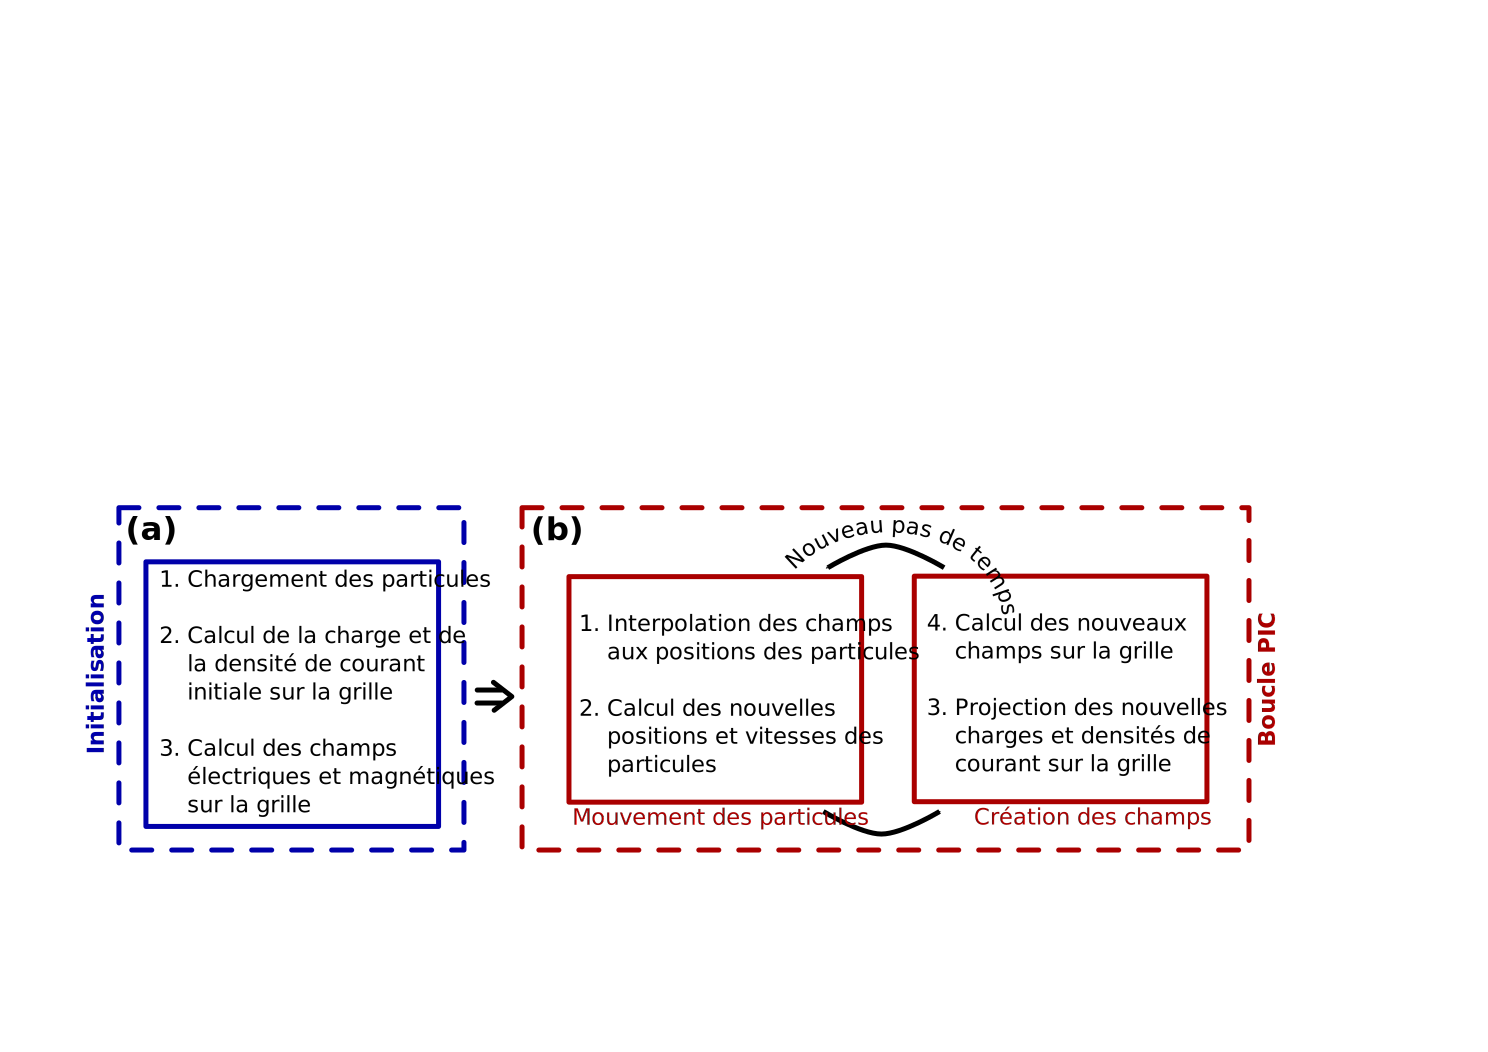
\includegraphics[width=\linewidth]{4-simulation/principe_PIC.png}
	\caption{Représentation schématique de l'algorithme d'un code PIC avec (a) les étapes principales de l'initialisation des macro-particules et des champs, et (b) les étapes principales de sa boucle temporelle.}
	\label{fig:4-PIC_algo}
\end{figure}

%\subsubsection{Conditions de bords}

Après que les nouvelles positions et vitesses des macro-particules aient été calculées, il est possible que ces dernières sortent de la boite de simulation. Elles peuvent alors être supprimées de la simulation, arrêtées dans la dernière maille, réfléchies selon une réflexion spéculaire, réinjectées depuis le bord opposé de la boite ou avec une impulsion tirée aléatoirement selon une loi Maxwellienne de température choisie à l'avance. 
De la même manière, les champs atteignant les bords de la boite peuvent être absorbés, réfléchis ou réinjectés au bord opposé de la boite.
Ces \textbf{conditions de bords} sont définies dans le fichier d'entrée de Smilei pour chaque bord et de manière indépendante pour les champs et chaque espèce de particule. 

Lors du calcul de l'évolution conjointe des champs et des particules, plusieurs \textbf{modules physiques additionnels} peuvent aussi être implémentés dans la simulation, tels que les collisions binaires entre particules, l'ionisation collisionelle ou l'ionisation par effet de champ (ionisation tunnel), ainsi que certains processus d'électrodynamique quantiques, tels que la production de photons par Compton Inverse multi-photon (ou \textit{synchrotron-like}) et la production de paires électron-positron par le processus Breit-Wheeler multi-photon. Pour le moment, les processus Bremsstrahlung et Bethe-Heitler ne sont cependant pas disponibles. Cette liste de module physique externes est néanmoins en constante évolution.
Les modèles de collisions binaires, d'ionisation collisionelle et d'ionisation par effet tunnel ont notamment été comparés à des résultats de modèles théoriques. Plus d'informations sont disponibles dans la documentation Smilei \parencite{derouillat_2018}.

Dans Smilei comme dans d'autres codes PIC, toutes les quantités physiques (charge, masse, énergie, champs électriques et magnétiques, …) sont normalisées à des quantités caractéristiques dépendantes de la pulsation du laser. Pour ne pas perdre en généralité, les quantités calculées à partir de ces codes sont donc souvent données en unités normalisées dans la littérature. Cependant, certains modules physiques externes de Smilei, comme par exemple l'ionisation par effet de champ, nécessitent que les unités physiques soient spécifiées dans la simulation. Dans ce cas, les simulations sont alors valides uniquement pour une pulsation laser bien définie. Puisque nous utiliserons ce type de module, dans le cadre de cette thèse nous spécifierons donc les quantités (distances, temps, …) en \textbf{unités physiques} usuelles (micromètres, picosecondes, …) et pas en unités du code.

\subsubsection{Diagnostics et outils d'analyse}

Afin de diminuer le volume de données à écrire sur le disque et faciliter leur analyse, Smilei est fourni avec des diagnostics pré-implémentés ainsi qu'un module d'analyse en \textit{Python} nommé happi. 
Ces derniers permettent d'étudier l'évolution des densités de charges, de courant et des champs dans la boite de simulation (via un \textit{DiagField}), ainsi que des quantités plus globales telles que l'énergie totale contenue dans la boite, ou l'énergie contenue dans les particules ou les champs (via un \textit{DiagScalar}). De plus, il est aussi possible de produire des histogrammes à partir des données de l'espace des phases, soit en considérant un instantané (temps fixé, via un \textit{DiagParticleBinning}), soit en intégrant temporellement une quantité à une position donnée (via un \textit{DiagScreen}).
Parmi les nombreux diagnostics disponibles, nous utiliserons principalement le diagnostic \textit{DiagField} permettant d'exporter les champs sur une grille prédéfinie, ainsi que le diagnostic \textit{DiagTrackParticles} permettant d'exporter l'espace des phases de particules satisfaisant une certaine condition. 

En géométrie 2D plane, la direction perpendiculaire au plan de simulation n'est pas simulée, et les poids statistiques des particules représentent un poids par unité de longueur et pas directement un nombre de particules. Le nombre de particules réelles peut être estimé en normalisant le poids statistique par une longueur caractéristique dans la dimension transverse, typiquement la taille de la tache focale du laser, ce qui reviens à supposer que la physique de l'interaction laser-plasma est relativement homogène sur cette longueur caractéristique.

Plus d'informations sur ces aspects sont disponibles dans la documentation officielle de Smilei \parencite{smilei_web}.

\subsection{Étude de paramètres numériques}

Dans la chaîne de simulations développée pour cette thèse, les simulations PIC sont les plus coûteuses en temps de calcul ; c'est pourquoi nous accordons ici un intérêt particulier à l'optimisation des paramètres numériques, en particulier la résolution spatiale et le nombre de particules par maille. De plus, cette étude nous permettra de nous assurer que les résultats obtenus ne varient pas significativement avec la résolution, le nombre de particules par maille, l'ordre d'interpolation ou l'ajout d'un module de collisions binaires.

\subsubsection{Définition des paramètres étudiés}

Nous considérons ici une situation typique où un laser d'\textbf{intensité $I_0=10^{20} \si{\W\per\cm^2}$} \textbf{polarisé linéairement}, de \textbf{longueur d'onde $1$ µm}, de \textbf{durée $30$ fs} (largeur à mi-hauteur) est focalisé avec une \textbf{tache focale de $5$ µm} (largeur à mi-hauteur) sur une \textbf{cible solide de polystyrène} $\rm (C_8 H_8)_n$ de densité électronique moyenne $300 ~ \rm n_c$, \textbf{d'épaisseur $15$ µm}, sur laquelle est collée un \textbf{absorbant homogène quasi-critique de polystyrène} de densité $0.96 ~ \rm n_c$ et d'épaisseur $11$ µm. Ces paramètres sont proches de ceux utilisés pour les simulations qui seront détaillées au chapitre \ref{chap:6-opti_numerique}. Ces paramètres et la géométrie de la simulation sont résumés en figure \ref{fig:4-PIC_boite_simu_validation}.

\begin{figure}[hbtp]
	\centering
	\includegraphics[width=0.5\linewidth]{4-simulation/boite_simu_validation.png}
	\caption{Dimensions caractéristiques de la boite de simulation PIC. Le laser se propage de gauche à droite, et les électrons sont exportés dans les 5 derniers µm du substrat.}
	\label{fig:4-PIC_boite_simu_validation}
\end{figure}

La simulation est effectuée dans une boite de \textbf{géométrie 2D plane} de $70$ µm $\times$ $70$ µm pendant $1$ ps. La cible est collée au bord arrière de la boite de simulation avec \textbf{conditions aux bords absorbantes} pour les particules et les champs électromagnétiques. 

La cible n'est \textbf{pas ionisée au début de la simulation}, et le \textbf{module d'ionisation par effet de champ} est \textbf{activé}. Les \textbf{atomes} sont aussi considérés parfaitement froids, et sont donc \textbf{immobiles avant l'arrivée du laser}. De cette manière, les particules proches des bords de la boite de simulation ne peuvent pas être absorbées par les conditions de bords avant d'avoir été influencées par le laser. Dans ce type de configuration, les électrons qui devraient physiquement être injectés dans le convertisseur collé au bord arrière du substrat (voir chapitre \ref{chap:3-methodes_exp}) sont donc supprimés de la simulation.

Les macro-électrons d'énergie cinétique supérieure à $m_e c^2$ sont exportés dès lors qu'ils se trouvent dans les $5$ derniers µm du substrat solide, en ne testant cette condition que tous les $5 ~ \si{\um/c} \approx 17 ~ \si{\fs}$ et en s'assurant de n'exporter chaque macro-particule qu'une seule fois par simulation (voir figure \ref{fig:4-PIC_boite_simu_validation}). Ce diagnostic permet de récupérer l'\textbf{espace des phases des électrons en face arrière du substrat} afin d'étudier les propriétés des sources d'électrons qui pourraient éventuellement être injectées dans des simulations \textit{Monte Carlo} du convertisseur, tel que cela sera effectué au chapitre \ref{chap:6-opti_numerique}. Les champs $\vec{E}$, $\vec{B}$ et les densités électroniques et ioniques sont aussi exportés dans une portion de la grille de $36$ µm $\times$ $30$ µm centrée sur l'axe de propagation laser et collée au bord droit, avec une résolution spatiale (mailles carrées) de $10$ mailles par longueur d'onde. L'export des champs et densités sur une grille plus petite que la grille de simulation permet de diminuer l'espace de stockage nécessaire à ce diagnostic.

L'\textbf{influence de la résolution spatiale} est étudiée, en considérant des mailles carrées ($\Delta y = \Delta x$) et une résolution temporelle fixée à $\Delta t = 0.95 \Delta x/\sqrt{2}$ de façon à satisfaire la condition Courant-Friedrichs-Lewy en géométrie 2D plane (voir équation (\ref{eq:4-PIC_CFL})). L'\textbf{influence du nombre d'ions par mailles} est elle aussi étudiée (il n'y a pas de macro-électrons au début de la simulation ; ceux-ci étant créés par ionisation).
Nous considérons un cas de référence avec une résolution spatiale de $60$ mailles par longueur d'onde, et avec $10$ macro-ions d'hydrogène ($\rm H$) et 10 macro-ions de carbone ($\rm C$) par maille. Un cas à haute résolution est aussi étudié, avec une résolution spatiale de $80$ mailles par longueur d'onde et 10 macro-ions (10 de $\rm H$ + 10 de $\rm C$) par mailles. L'\textbf{influence de l'ordre d'interpolation}, ainsi que l'effet des \textbf{collisions électrons-ions} (avec ionisation collisionnelle) est aussi étudiée pour le cas à haute résolution. Ce dernier cas est donc le plus précis, et nous permettra de déterminer s'il est possible de retrouver des résultats similaires avec des simulations plus rapides (résolution et nombre de macro-ions par maille plus faible, collisions désactivées). 

Les simulations ont été lancées sur 20 noeuds manycores (64 coeurs par noeud, soit 1280 coeurs au total) de la partition Irene-KNL du super-calculateur TGCC Joliot-Curie (CEA Bruyères-le-Châtel) avec 4 processus \textit{MPI} par noeud (soit 16 coeurs par processus \textit{MPI}) et 32 threads \textit{OpenMP} par processus \textit{MPI} (hyper-threading conseillé par J. Derouillat de l'équipe de Smilei sur cette machine). La boite de simulation est découpée en $128 \times 128$ patches (environ 6 patches par thread) avec un load balancing toutes les 20 itérations. Afin de satisfaire le découpage en patches pour toutes les simulations, la taille de la boite de simulation est automatiquement ajustée en ajoutant du vide devant la cible. La version de Smilei utilisée est la version 4.5, et la vectorisation n'a pas été activée. Plus de détails sur les techniques de parallélisation sont disponibles dans la documentation de Smilei \parencite{smilei_web}, et le vocabulaire utilisé est défini (en anglais) en référence \parencite{vocab_parallelisation}. 

\subsubsection{Temps de calcul et convergence des résultats}

Le tableau \ref{tab:4-temps_calcul_PIC} résume les paramètres numériques utilisés pour cette étude, et indique le temps de calcul correspondant, en heure CPU (hCPU), pour toutes ces simulations. Les diagnostics de champs occupent un espace de stockage d'environ $800$ Mo pour chaque simulation, tandis que le diagnostic d'espace des phases des particules nécessite entre $200$ Mo (pour le cas \textit{IV}) et $5$ Go de stockage (pour le cas \textit{VII}). L'espace stockage nécessaire pour les autres fichiers de diagnostics est négligeable.
Le \textbf{temps de calcul} est \textbf{très dépendant de la résolution et du nombre de macro-particules par mailles} ; un plus grand nombre de macro-ions par maille et une résolution plus importante (donc un nombre de mailles plus important) nécessitant plus d'opérations de calcul. L'utilisation d'un ordre d'interpolation de $2$ diminue le temps de calcul de $40 \%$ pour le cas à haute résolution, alors que l'activation du module de collisions l'augmente d'un facteur $>2$. Pour le cas de référence, diviser le nombre de particules par $2$ permet de diminuer le temps de calcul de $40 \%$ tandis que diviser le nombre de particules par $10$ diminue le temps de calcul d'un facteur $> 4$.

\begin{table}
\centering
\begin{tabular}{ | l | l | l | l | l || l | }
    \hline
            & Résolution    & Nombre        & Ordre             & Collisions    & Temps total \\
    Label   & spatiale      & d'ions/maille & d'interpolation   & activées      & en hCPU \\
    \hline
    \textit{I}   & 40 mailles/$\lambda_L$ & 10          & 4         & Non        & 1583     \\
    \textit{II}  & 60 mailles/$\lambda_L$ & 10          & 4         & Non        & 3866     \\
    \textit{III} & 60 mailles/$\lambda_L$ & 5           & 4         & Non        & 2224     \\
    \textit{IV}  & 60 mailles/$\lambda_L$ & 1           & 4         & Non        & 899      \\
    \textit{V}   & 80 mailles/$\lambda_L$ & 10          & 4         & Non        & 8054     \\
    \textit{VI}  & 80 mailles/$\lambda_L$ & 10          & 2         & Non        & 5847     \\
    \textit{VII} & 80 mailles/$\lambda_L$ & 10          & 4         & Oui        & 18496    \\
    \hline
    \end{tabular}
    \caption{Définition des paramètres numériques étudiés, et temps de calcul correspondant. Le cas de référence est le cas \textit{II}, et le cas à haute résolution est le cas \textit{V}. Les autres cas présentent des variations par rapport à ces derniers.}
	\label{tab:4-temps_calcul_PIC}
\end{table}


L'analyse de l'énergie totale contenue dans la boite nous permet d'étudier le chauffage numérique éventuel des électrons. L'évolution de l'énergie totale dans la boite de simulation, ainsi que l'énergie cinétique contenue dans toutes les espèces (électrons et ions) est tracée en fonction du temps en figure \ref{fig:4-PIC_chauffage_numerique}. Pour chacune de ces simulations, l'énergie totale augmente au début de la simulation à cause de l'injection du laser dans la boite. Nous pouvons ensuite observer que la physique du \textbf{transfert d'énergie} entre le laser et le plasma (autour de $(50 ~ \si{[\um/c]} + \tau_{FWHM}) \sim 0.2$ ps) semble assez \textbf{similaire} pour ces différents cas. Aux \textbf{temps plus longs}, on observe cependant pour certaines simulations que l'\textbf{énergie cinétique des espèces augmente avec le temps}, faisant aussi augmenter l'énergie totale contenue dans la boite. Ce type de comportement non physique est caractéristique du phénomène de \textbf{chauffage numérique}.
Nous pouvons aussi observer que pour le cas à haute résolution sans collisions \textit{V}, les \textbf{énergies cinétiques et totales} tendent plutôt à légèrement \textbf{diminuer avec le temps}. Ceci peut être expliqué qualitativement comme la conséquence des \textbf{conditions aux bords absorbantes} pour les particules et les champs, qui peuvent sortir de la boite et emporter une partie de l'énergie avec eux. Le cas de référence \textit{II} ainsi que son équivalent avec 5 macro-ions par maille \textit{III} et le cas à plus basse résolution \textit{I} sont superposés au cas \textit{V}.
Lorsque le nombre de macro-ions par mailles est faible, comme pour le cas de référence avec $1$ macro-ion par maille \textit{IV}, l'énergie totale dans la boite semble surestimée aux temps longs et on observe un léger chauffage numérique. L'ordre d'interpolation semble aussi jouer un rôle important car, même avec la plus haute résolution et $10$ macro-ions par mailles, la simulation \textit{VI} comprenant un ordre d'interpolation de $2$ subit du chauffage numérique aux temps longs. Le module de collisions semble aussi jouer un rôle non négligeable dans le chauffage numérique des électrons aux temps longs, comme nous pouvons le remarquer sur la courbe du cas \textit{VII}. 

\begin{figure}[hbtp]
	\centering
	\includegraphics[width=0.7\linewidth]{4-simulation/comparaison_U.png}
	\caption{Comparaison des énergies totales (traits pleins) et cinétiques (traits pointillés) contenues dans toute la boite de simulation, pour les différentes simulations étudiées. Les cas \textit{I},\textit{II}, \textit{III} et \textit{V} sont superposés.}
	\label{fig:4-PIC_chauffage_numerique}
\end{figure}

Nous pouvons ensuite traiter l'espace des phases des \textbf{électrons exportés en face arrière du substrat avec une énergie cinétique supérieure à $m_e c^2$} afin de comparer leurs distributions en énergie, leurs distributions en angle polaire, leurs distributions spatiales transverse ainsi que leurs temps d'export dans le diagnostic (affichés respectivement en figures \ref{fig:4-PIC_validation_electrons}a, \ref{fig:4-PIC_validation_electrons}b, \ref{fig:4-PIC_validation_electrons}c et \ref{fig:4-PIC_validation_electrons}d).
Le cas \textit{IV} comprenant le moins de particules par maille est le plus dispersé en queue de distribution en énergie et en angle. Il est aussi spatialement moins piqué, et la charge totale du faisceau d'électrons (donc leur nombre total, non représenté ici) est inférieure aux autres cas (65 nanocoulombs contre 70 à 75 nanocoulombs pour les autres simulations). 
Tous les autres cas sont quantitativement assez proches pour ces diagnostics. En particulier, nous pouvons donc en conclure que l'effet des collisions est relativement limité dans ce type de simulations. Compte tenu de la similarité de ces résultats lorsque nous considérons uniquement les électrons \textbf{exportés dans le diagnostic} et dont \textbf{l'énergie cinétique est supérieure à $m_e c^2$}, nous pouvons en déduire que les effets de \textbf{chauffage numérique} précédemment décrits concernent principalement les \textbf{électrons qui sont peu énergétiques et ne sont pas éjectés en face arrière de la cible}. 
Nous pouvons observer que, pour ces électrons, la distribution spatiale transverse du faisceau est relativement piquée autour de l'axe de propagation, ce qui semble montrer que la taille transverse de la boite de simulation est suffisamment importante. Une distribution spatiale plus plate aurait en effet au contraire indiqué qu'un nombre non négligeable d'électrons aurait pu quitter la boite sur les bords avant d'être exporté en face arrière du substrat. 
Le nombre d'électrons d'énergie cinétique supérieure à $m_e c^2$ exportés est relativement négligeable après $0.8$ ps, ce qui semble indiquer que l'interaction du laser avec la cible a été décrite suffisamment longtemps pour ces particules et que le temps de simulation choisi est suffisamment important. 

\begin{figure}[hbtp]
	\centering
	\includegraphics[width=\linewidth]{4-simulation/Smilei_validation.png}
	\caption{Comparaison de différentes caractéristiques des sources d'électrons pour les différentes simulations étudiées, avec (a) leurs distributions en énergie, (b) leurs distributions angulaire, (c) leurs distributions spatiale transverse et (d) leurs distributions temporelle.}
	\label{fig:4-PIC_validation_electrons}
\end{figure}

Compte tenu des résultats très similaires obtenus pour les sources d'électrons avec ces différents paramètres de simulations, le cas à faible résolution avec 10 macro-ions (10 $\rm C$ + 10 $\rm H$) par maille \textit{I}, ou le cas de référence avec 5 macro-ions par mailles \textit{III} seraient a priori suffisants pour cette situation, et il ne serait pas très intéressant d'utiliser une résolution importante comme le cas \textit{V}. L'utilisation d'un ordre d'interpolation de $2$ avec le cas \textit{VI} ou d'un seul macro-ion par maille avec le cas \textit{IV} permet de faire diminuer le temps de calcul mais augmente le chauffage numérique. L'utilisation du module de collisions dans le cas \textit{VI} augmente considérablement le temps de calcul et n'amène pas de modifications significatives de nos résultats.
Afin de bénéficier d'une bonne statistique, les paramètres de notre cas de référence avec 10 macro-ions par maille \textit{III} seront utilisés comme base pour l'étude que nous mènerons au chapitre \ref{chap:6-opti_numerique}, où ce type de simulation sera aussi analysé plus en détails.

\section{Modélisation de la propagation de particules dans la matière}

Une fois que des électrons ont été accélérés par le laser, nous cherchons à les injecter dans un convertisseur afin de transférer une partie significative de leur énergie cinétique en photons $\gamma$.

\newpage

Comme nous l'avons vu au chapitre \ref{chap:1-particules}, la longueur caractéristique de perte d'énergie par rayonnement est nommée longueur de radiation, et est de l'ordre de quelques millimètres pour des matériaux de densité et numéro atomique élevés (e.g. $\sim 3 ~ \si{\mm}$ pour du platine). Pour ce type de matériaux et d'épaisseurs, nous nous attendons aussi à ce que les effets collisionnels jouent un rôle majeur pour la propagation des électrons dans le convertisseur (voir chapitre \ref{chap:1-particules}).
Ainsi, bien que les codes PIC puissent en théorie être utilisés pour simuler la propagation d'électrons dans le convertisseur, ce type d'épaisseurs est prohibitif en terme de temps de calcul, en particulier pour des simulations à 2 ou 3 dimensions de matériaux denses (nécessitant donc une résolution importante), et avec des modules physiques de collisions activés.

Au contraire, la propagation de particules dans la matière dans des régimes collisionnels est très souvent étudiée à l'aide d'algorithmes de transport de type \textit{Monte Carlo} (noté MC), où les épaisseurs de solide simulées peuvent facilement atteindre plusieurs centimètres voire mètres \parencite{agostinelli_2003}. Pour ce type d'applications, cette approche est \textbf{beaucoup moins coûteuse en temps de calcul} que les codes PIC ou hybrides, et peut donc permettre d'étudier une grande variété de matériaux et d'épaisseurs de convertisseurs en un temps raisonnable. Ces codes reposent cependant sur l'hypothèse que \textbf{le matériau n'est pas modifié par le passage des particules} (la densité et les sections efficaces sont constantes), et que les \textbf{particules injectées} peuvent être considérées \textbf{indépendantes les unes des autres}. Ainsi, pour utiliser ce type de méthode il doit être possible de considérer que les \textbf{effets collisionnels} sont \textbf{dominants sur les effets collectifs} lors de la propagation du faisceau (à l'opposé des codes PIC dont l'intérêt réside justement dans la modélisation de ces effets collectifs et où les collisions sont par défaut négligées).

Dans l'étude numérique que nous mènerons au chapitre \ref{chap:6-opti_numerique}, les électrons accélérés dans le code PIC Smilei seront injectés dans une application Monte Carlo nommée gp3m2 (présentée dans cette section) qui nous permettra de simuler leur propagation dans le convertisseur. Pour transférer les électrons simulés via le code PIC dans le code MC, nous choisirons de \textbf{simuler le substrat dans ces deux codes}, et d'\textbf{injecter les particules dans le code MC à leur position d'export dans le code PIC} (voir figure \ref{fig:4-MC_PIC_transition}), avec leur \textbf{impulsion et temps correspondant}. 

\newpage 

Dans ce type de situations, les hypothèses inhérentes à la méthode Monte Carlo nous contraignent néanmoins à supposer que le faisceau d'électrons a un comportement différent dans les deux types de simulations, malgré des caractéristiques identiques (même espace des phases). Pour la propagation des électrons dans un convertisseur froid, dense et de numéro atomique élevé, on peut néanmoins justifier cette hypothèse qualitativement en notant que, dans ce type de matériau, la propagation du faisceau est très fortement influencée par les diffusions, car celles-ci y sont très fréquentes (voir chapitre \ref{chap:1-particules}). Ces effets collisionnels tendent par conséquent à limiter l'importance relative des effets collectifs.
L'effet des \textbf{champs électromagnétiques} en face avant de la cible ainsi que le \textbf{courant de retour d'électrons froids} sont eux aussi \textbf{négligés dans le convertisseur}, bien qu'ils puissent jouer un rôle significatif dans la propagation des électrons énergétiques dans la matière \parencite{davies_1997, compantlafontaine_2018}. Pour un convertisseur suffisamment épais, on s'attend à ce que le phénomène d'écrantage atténue l'effet des champs électromagnétiques situés hors du convertisseur, et limite donc leur influence sur la propagation du faisceau de particules. La justification rigoureuse de ces hypothèses nécessiterait néanmoins une étude approfondie. Différents aspects de ce problème sont discutés notamment dans les références \parencite{davies_2002, tikhonchuk_2002, davies_1997, compantlafontaine_2018}. 

\begin{figure}[hbtp]
	\centering
	\includegraphics[width=0.7\linewidth]{4-simulation/transition_PIC_MC.png}
	\caption{Schéma de principe du transfert de données entre les codes Particle-In-Cell et Monte Carlo. Les particules enregistrées dans le substrat dans le code PIC sont réinjectées à leur position d'export dans le code Monte Carlo.}
	\label{fig:4-MC_PIC_transition}
\end{figure}

Dans cette section, nous étudierons tout d'abord le principe de base d'un algorithme de transport \textit{Monte Carlo}, ainsi que les spécificités des outils Geant4. Nous présenterons ensuite l'application gp3m2 développée dans le cadre de cette thèse. Celle-ci sera utilisée au chapitre \ref{chap:6-opti_numerique} pour simuler la production d'une sources de photons $\gamma$ via le processus Bremsstrahlung, et en utilisant la méthode décrite précédemment pour le transfert de données depuis le code PIC. Cette application est néanmoins adaptée à un grand nombre d'autres situations, tel que cela sera notamment évoqué au chapitre \ref{chap:6-opti_numerique}. 

\subsection{Principe des outils \textit{Monte Carlo} Geant4}

Geant4 (pour GEometry ANd Tracking) est un ensemble d'outils logiciels pour l'étude numérique de la propagation de particules dans la matière. Ses domaines d'applications incluent la physique des hautes énergies et des accélérateurs, la physique nucléaire, médicale ou encore l'astrophysique.



Ces outils open-source sont développés en \textit{C++} orienté objet par une large collaboration internationale, et implémentent de nombreuses fonctionnalités pour la production d'une application \textit{Monte Carlo}. La philosophie très modulaire de Geant4 lui permet d'être applicable à un grand nombre de situations différentes, notamment en termes de processus et de modèles physiques (traitement des énergies de quelques eV à plusieurs TeV), selon des géométries complexes, et avec des sources de particules primaires et des diagnostics personnalisables. Bien que de nombreux exemples d'applications soient fournis avec le code source, aucun n'était néanmoins adapté au traitement complet de l'espace des phases aussi bien en entrée qu'en sortie de code. Une application nommée gp3m2 (pour Geant4 simulation of Particle Phase-space Propagation in a Multi-layer Material) a donc été développée durant cette thèse pour répondre à ce besoin.


Plus d'informations sur les outils Geant4 sont disponibles dans les références \parencite{agostinelli_2003, allison_2006, allison_2016}. Une documentation pratique est aussi disponible sur son site officiel \parencite{geant4_web}, où il est notamment possible de consulter les \textit{Physics Reference Manual} et \textit{Application Developper Guide}. Ces documents, dont la prochaine section est en partie inspirée, permettent de se renseigner respectivement sur la physique simulée et sur la façon d'implémenter les classes Geant4 dans sa propre application. Une documentation pour l'application gp3m2 est disponible sur son dépot github \parencite{gp3m2}. Plus d'informations sur la méthode \textit{Monte Carlo} peuvent notamment être trouvées dans la référence \cite{haghighat_2015}.

\subsubsection{Algorithme \textit{Monte Carlo} pour le transport de particules}

Dans un code \textit{Monte Carlo} de transport de particules (abrégé en code \textit{Monte Carlo}, ou code MC), les particules injectées dans la simulation sont appelées \textit{particules primaires}, tandis que celles produites lors de processus physiques sont appelées \textit{particules secondaires}. Afin de limiter le nombre de particules simulées, ces codes se basent eux aussi sur un échantillonnage de la fonction de distribution via des \textbf{macro-particules} auxquelles sont assignés un \textbf{poids statistique arbitraire}. Ces dernières n'ont cependant pas de facteur de forme spatial comme pour les codes PIC. Le nombre de macro-particules $N$ doit être suffisamment important pour correctement échantillonner la fonction de distribution, et le rapport signal sur bruit varie en $\sqrt{N}$ \parencite{haghighat_2015}.

Lorsque ces particules (primaires ou secondaires) se propagent dans la matière, elles peuvent interagir avec le milieu environnant par l'intermédiaire de différents processus, dont les plus significatifs ont été évoqués au chapitre \ref{chap:1-particules} (ionisation, diffusions élastiques, etc ...). La probabilité d'interaction de chaque processus est usuellement modélisée par une section efficace notée $\sigma$, et ces \textbf{interactions} sont supposées \textbf{ponctuelles} et \textbf{indépendantes} les unes des autres.

Dans ce cas, il est possible de montrer (voir chapitre 2 de la référence \parencite{rax_2007}) que la probabilité de \textbf{ne pas interagir pendant une distance $\ell$} est donnée par \parencite{geant4_physref, haghighat_2015} :
\begin{equation}
    P(\ell)= \exp\left(-\dfrac{\ell}{\ell_{int}}\right)~ \rm ,
\end{equation}
où $\ell_{int}$ est une longueur d'interaction typique \textbf{pour ce processus dans ce matériau} aussi appelée \textit{libre parcours moyen}, et qui s'exprime comme :
\begin{equation}
    \ell_{int} = \dfrac{1}{n ~ \sigma} ~ \rm ,
\end{equation}
avec $\sigma$ la section efficace du processus considéré, et $n$ la densité de particules cibles dans le matériau.
Dans les codes Monte Carlo, un tirage aléatoire permet alors de générer une distance de parcours \textbf{pour ce processus dans ce matériau} via \parencite{haghighat_2015} :
\begin{equation}
    \ell = - \ell_{int} \times \ln{\eta} ~ \rm ,
\end{equation}
où $\eta$ est une variable aléatoire uniforme dans $[0,1[$.

Lors de la création d'une particule simulée, une longueur de parcours $\ell$ est tirée aléatoirement \textbf{pour chaque processus}, chacun ayant un libre parcours moyen et un état final potentiellement différents (dépot d'énergie, création de particules secondaires, ...). Le processus effectivement mis en oeuvre est alors celui ayant \textbf{la distance la plus courte}, et les autres longueur de parcours sont ensuite modifiées pour prendre en compte la distance déjà parcourue, notée ici $\Delta \ell$ \parencite{haghighat_2015}. L'intervalle entre deux interactions physiques est appelé \textit{Step} dans le langage de Geant4. Cet algorithme est représenté schématiquement en figure \ref{fig:4-MC_algo}. 

\begin{figure}[hbtp]
	\centering
	\includegraphics[width=\linewidth]{4-simulation/principe_MC.png}
	\caption{Principe d'un code \textit{Monte Carlo}, où (a) les libres parcours moyens sont calculés lors de initialisation, puis (b) une distance au prochain point d'interaction est tirée aléatoirement en fonction du libre parcours moyen. Le processus ayant la distance la plus courte est choisi et mis en œuvre, puis (c) une nouvelle distance est tirée pour ce processus pendant que les distances au point d'interaction sont mises à jour pour les autres processus. Le processus ayant la distance la plus courte est alors mis en œuvre, et l'étape (c) recommence.}
	\label{fig:4-MC_algo}
\end{figure}

Dans Geant4, le tirage aléatoire est en fait effectué non pas sur la distance de parcours $\ell$ du \textit{Step} courant, mais plutôt sur le \textbf{nombre de libre parcours moyens} correspondant $N_{\ell_{int}}$ (cette astuce permet notamment de faciliter le calcul de la distance de parcours lors d'un changement de matériau) \parencite{geant4_physref, agostinelli_2003} :
\begin{equation}
    N_{\ell_{int}}=\dfrac{\ell}{\ell_{int}} = - \ln\eta ~ \rm ,
\end{equation}
et après chaque étape de calcul, pour chaque processus le nombre de libre parcours moyen restants $N_{\ell_{int}}'$ est alors mis à jour \parencite{geant4_physref} :
\begin{equation}
    N_{\ell_{int}}'=N_{\ell_{int}} - \dfrac{\Delta \ell}{\ell_{int}} ~ \rm ,
\end{equation}
ainsi que le temps associé à la particule (dans le référentiel du laboratoire) \parencite{geant4_physref} :
\begin{equation}
    t_f = t_i +  \dfrac{\Delta \ell}{2}\left(\dfrac{1}{v_i}+\dfrac{1}{v_f}\right) ~ \rm ,
\end{equation}
avec $v_i$ et $v_f$ les vitesses de la particule respectivement au point d'interaction précédent et au point d'interaction courant, et $t_i$ et $t_f$ les temps correspondant respectivement à l'interaction précédente et courante.

Le parcours des particules est aussi arrêté par les interfaces entre différent matériaux, et plus généralement lors de tout changement de volume défini dans la simulation (appelé \textit{volume logique}) sans forcement qu'il y ait changement de matériau. Ce comportement sera d'ailleurs mis à profit dans notre application décrite dans la prochaine section.

Ces étapes de calcul sont répétées de la création à la destruction de la particule simulée. 

\subsubsection{Processus et modèles physiques}

Dans certains cas, simuler toutes les interactions discontinues (ou discrètes) des particules lors de leur propagation n'est néanmoins pas très efficace, et certaines techniques permettent d'améliorer le temps de calcul. 
En effet, lorsque des particules se propagent dans la matière, elles peuvent produire un très grand nombre de particules secondaires, par ionisation par exemple. Nombre de ces particules secondaires sont cependant très peu énergétiques, et se propagent donc sur une distance très faible (voir chapitre \ref{chap:1-particules}). Dans Geant4, une distance appelée \textit{range cut} est donc définie par l'utilisateur, et les particules secondaires n'ayant que très peu de chances de se propager sur cette distance caractéristique ne sont pas générées \parencite{geant4_physref}. Cette technique permet ainsi de diminuer grandement le nombre de particules secondaires à simuler, et l'énergie emportée par ces particules est simplement considérée comme une \textbf{perte d'énergie continue} pour la particule incidente \parencite{geant4_physref}. 
De plus, pour les processus très fréquents impliquant une variation d'énergie faible et une déviation angulaire faible, tels que la perte d'énergie par ionisation ou les diffusions multiples pour les électrons (voir chapitre \ref{chap:1-particules}), il est numériquement très coûteux de simuler individuellement chaque interaction de la particule incidente avec la matière, et ces processus sont aussi considérés comme \textbf{continus} \parencite{geant4_physref}. L'effet des diffusions multiples est quant à lui calculé et ajouté à la trajectoire de la particule à la fin de chaque \textit{Step} \parencite{geant4_physref}. 
La plupart des autres processus (Bremsstrahlung, création de paires, ...) sont néanmoins décrits de façon discrète, tel que cela a été présenté précédemment.
D'autres techniques plus avancées (roulette russe, biaising, ...) permettent aussi d'améliorer la convergence du calcul mais ne seront pas discutées dans le cadre de cette thèse.

Ces différents processus, discrets ou continus, sont implémentés par différents modèles théoriques, semi-empiriques, ou jeux de données expérimentales. Bien qu'il soit possible à l'utilisateur de choisir quels modèles utiliser dans quelles conditions (et même d'ajouter ses propres processus et modèles), Geant4 propose toutefois des \textbf{listes de processus physiques et de modèles déjà définis} et adaptés à différentes situations physiques et gammes d'énergies, comme par exemple la physique des photons optiques, des interactions électromagnétiques, ou de la décroissance des particules instables. Certaines de ces listes (appelées \textit{reference PhysicsLists} dans Geant4) ont de plus été activement validées contre des données expérimentales \parencite{geant4_val}.

Les propriétés de la plupart des matériaux et de la plupart des particules sont aussi déjà implémentées dans ces outils de base, mais il est toujours possible d'ajouter de nouveaux matériaux ou particules si besoin.

\subsubsection{Autres fonctionnalités}

En plus de la gestion des processus physiques et du transport des particules, Geant4 propose de nombreux outils permettant de s'adapter à des contextes très variés. Nous mentionnerons simplement les outils pour la création d'une \textbf{géométrie}, où les volumes de matières peuvent être définis à partir de volumes simples (pavés, cylindres, …) et d'opérations entre ceux ci (répétitions, union, différence, …), ainsi que des outils pour la \textbf{définition des propriétés des particules primaires}, la production semi-automatisée d'histogrammes pour l'\textbf{analyse des données générées par la simulation}, ou encore des outils de \textbf{visualisation} de la trajectoire des particules, ... Plus d'informations sont disponibles dans la référence \parencite{geant4_appdev}.


\subsection{Présentation de l'application gp3m2}

Pour produire une source de photons $\gamma$ adaptée à l'étude du processus BWL, nous aurons besoin d'optimiser l'épaisseur de convertisseurs pour chaque source d'électrons produite dans nos simulations PIC. Nous chercherons donc à définir les propriétés des particules primaires injectées dans notre application Monte Carlo à partir de l'espace des phases des électrons générés par le code PIC (voir figure \ref{fig:4-MC_PIC_transition}). Pour pouvoir réutiliser les données générées dans d'autres codes (notamment le code TrILEns présenté dans la section suivante), il nous sera aussi nécessaire d'exporter l'\textbf{espace des phases des particules} qui \textbf{sortent du convertisseur}.

Pour répondre à ces objectifs, une application nommée gp3m2 a été développée dans le cadre de cette thèse à partir des outils Geant4, et est disponible en open source avec une documentation sur le dépot github \parencite{gp3m2}.

\subsubsection{Physique simulée}

Dans cette application, le convertisseur est considéré \textbf{cylindrique}, et est placé au centre d'une boite vide (matériau \textit{G4\_Galactic}) de dimensions 1 m $\times$ 1 m $\times$ 1 m.

Dans toutes nos simulations nous utiliserons la liste de processus physique (\textit{reference physics list}) nommée \textit{G4EmStandard\_option4}, car elle est considérée comme étant la plus précise pour les interactions électromagnétiques dans une large gamme d'énergie (de 1 keV à 100 TeV) \parencite{geant4_physref}. Parmi les processus implémentés les plus importants, nous pouvons notamment mentionner les diffusions multiples, l'ionisation, la production de photons par Bremsstrahlung et l'annihilation pour les électrons et les positrons, ainsi que la photo-ionisation, les diffusions Rayleigh, Compton et la production de paires électron-positron pour les photons (voir chapitre \ref{chap:1-particules}).

Sauf indications contraires le \textit{range cut} est fixé à 10 µm, et les propriétés des matériaux utilisés sont définies à partir des données du NIST, implémentées par défaut dans Geant4.

\subsubsection{Injection des particules primaires}

Afin de pouvoir étudier une large gamme de sources d'électrons différentes, les \textbf{propriétés des particules primaires} sont définies \textbf{à partir d'un fichier d'espace des phases}, qui est lu au début de la simulation. Ce type de fichier peut être \textbf{produit à partir de données de simulations PIC} par exemple, mais peut aussi être \textbf{généré à partir de distributions en énergie, en angle, en espace et en temps} déterminées, notamment via certains outils du module p2sat (module présenté à la fin de ce chapitre).

Dans ce fichier, la première colonne correspond au le poids statistique $w$ des macro-particules, tandis que la seconde, troisième et quatrième colonne contiennent respectivement les positions $x$, $y$, $z$ des particules. Les trois colonnes suivantes contiennent quant à elles la projection des impulsions des macro-particules selon $x$, $y$, $z$ notées $p_x$, $p_y$, $p_z$, et la dernière correspond au temps $t$ auquel ces informations ont été exportés. \textbf{Chaque ligne} de ce fichier décrit donc \textbf{une macro-particule}, et son \textbf{numéro de ligne} est un nombre entier qui peut permettre de \textbf{l'identifier}.

Lors de la création des particules primaires, nous définissons leurs poids statistiques, positions, impulsions et temps selon un \textbf{tirage aléatoire dans la liste de macro-particules du fichier d'entrée}. Nous générons donc aléatoirement un identifiant de particule ($\approx$ numéro de ligne), et définissons les propriétés des particules primaires à partir de la macro-particule correspondante. Ce type de tirage est \textbf{indépendant du poids statistique} de la macro-particule considérée, et \textbf{permet de bien représenter les configurations avec un poids statistique faible}. Les poids statistiques ayant été préalablement normalisés pour indiquer un nombre de particules réelles, il nous est aussi nécessaire de diviser chacun des poids $w$ par le nombre total de macro-particules tirées lors de la simulation, afin de conserver le nombre total de particules réelles représentées dans la simulation, et ce indépendamment du nombre de particules primaires simulées.

Pour un calcul parallélisé sur $N$ coeurs ce fichier est lu et sauvegardé en mémoire $N$ fois, et il sera donc nécessaire de veiller à ne pas fournir un fichier d'entrée trop lourd pour les capacités de la machine utilisée. Un algorithme de réduction de données d'espace des phases a été développé notamment pour cet effet, et celui-ci sera présenté à la fin de ce chapitre. De futurs développements pourraient permettre de limiter l'espace mémoire nécessaire en ne lisant qu'une seule fois le fichier d'entrée, et en partageant les informations entre les différents coeurs.

\subsubsection{Diagnostics}

Les particules primaires ainsi définies vont donc pouvoir interagir avec le convertisseur via les processus considérés dans la liste de processus physique. Pour une source d'électrons injectée donnée, nous pourrons chercher à optimiser les caractéristiques des sources de photons $\gamma$ produites en faisant varier l'épaisseur du convertisseur. Il nous serait aussi intéressant de pouvoir estimer les propriétés des sources d'électrons et positrons produits, qui pourraient contribuer au bruit de mesure expérimental. 

Pour récupérer ces informations, \textbf{l'espace des phases} (poids statistique, impulsion, position et temps) \textbf{de chaque particule} (photon $\gamma$, $e^-$, $e^+$) \textbf{s'échappant de la cible est sauvegardé}. Plus précisément, nous enregistrons l'espace des phases de chaque particule dès lors que celle-ci est arrêtée par un changement de volume logique, en effectuant un test à chaque \textit{Step}. De cette façon, l'espace des phases des particules d'un type donné est exporté \textbf{dans le même fichier}, et ce \textbf{indépendamment de sa position d'export} (par la face arrière du convertisseur, sa face avant ou ses bords). La détermination des propriétés de la source de particules éjectés spécifiquement en face arrière devra être effectuée en \textbf{post-traitement}, en filtrant les particules par leur position d'export. Ce type de géométrie est illustré par exemple en figure \ref{fig:4-MC_tranches_gp3m2}a, où les bords et la face avant du convertisseur ne sont pas représentés par souci de simplicité.

Pour une source d'électrons et un matériau donné, nous pouvons alors imaginer \textbf{optimiser l'épaisseur du convertisseur} en comparant les résultats obtenus par un \textbf{nombre $N$ de simulations différentes}, \textbf{en faisant} par exemple \textbf{varier l'épaisseur du convertisseur} de $0$ à $L$ ($L$ étant l'épaisseur maximale considérée) avec un pas constant de $\Delta L = L/N$. 
Bien que cette approche puisse être en principe suffisante, une \textbf{précision importante sur l'épaisseur} optimale du convertisseur ($\Delta L$ faible) nécessiterait un \textbf{nombre de simulations important}, et ce type de simulations serait relativement \textbf{peu efficace en terme de temps de calcul}.

Pour expliquer ceci, considérons tout d'abord une optimisation simplifiée avec seulement deux épaisseurs de convertisseurs $\Delta L$ et $2 \Delta L$. Dans la première simulation d'épaisseur $\Delta L$, représentée en figure \ref{fig:4-MC_tranches_gp3m2}a, des électrons sont injectés dans le convertisseur, se propagent et interagissent avec le matériau (dépôt d'énergie, diffusions, production de particules secondaires, ...). Les particules (primaires comme secondaires) ayant atteint la face arrière du convertisseur après avoir traversé une épaisseur $\Delta L$ de matière sont exportées puis sortent de la boite de simulation et sont détruites (on néglige l'export par la face avant ou par les bords pour cette explication par souci de clarté, même si cela ne change rien au fond du propos). De la même manière, dans la simulation d'épaisseur $2 \Delta L$ illustrée en figure \ref{fig:4-MC_tranches_gp3m2}b, les particules injectées se propagent, peuvent éventuellement produire des particules secondaires, et ces particules seront exportées puis détruites après avoir traversé une épaisseur $2 \Delta L$ de matière. Néanmoins, puisque les interactions dans la matière sont considérées \textbf{indépendantes} les unes des autres, nous pouvons considérer que, aux fluctuations statistiques près, les \textbf{propriétés des faisceaux de particules} se propageant dans les deux convertisseurs sont \textbf{similaires dans les deux simulations à une profondeur $<\Delta L$ donnée}. Pour ces profondeurs, la propagation de ces particules est donc simulée $2$ fois (1 fois par simulation) et \textbf{coûte donc du temps de calcul sans améliorer la précision des résultats}. L'ajout d'une troisième simulation d'un convertisseur d'épaisseur $3 \Delta L$, illustré en figure \ref{fig:4-MC_tranches_gp3m2}c, rendrait cette optimisation encore moins efficace, puisque la propagation des particules serait simulée 3 fois de $0$ à $\Delta L$, et $2$ fois de $\Delta L$ à $2 \Delta L$. Pour éviter ce type de problème, une solution pourrait être de récupérer les particules sortant en face arrière du convertisseur d'épaisseur $\Delta L$, et de les réinjecter à la profondeur $\Delta L$ dans une cible d'épaisseur $2 \Delta L$. De cette manière, la propagation des particules de $0$ à $\Delta L$ ne serait simulée qu'une seule fois (dans la simulation où l'épaisseur du convertisseur est $\Delta L$) et leur propagation de $\Delta L$ à $2\Delta L$ serait elle aussi simulée une seule fois (dans la simulation du convertisseur d'épaisseur $2\Delta L$). 

Afin de simplifier ce type de manipulations, le principe de notre application gp3m2 consiste en la simulation d'un convertisseur d'épaisseur $L$ découpé en $N$ tranches d'épaisseurs $\Delta L = L/N$. L'espace des phases des particules y est exporté à l'interface entre chacune des tranches, et il est ainsi possible de déterminer les propriétés des sources de particules produites \textbf{en fonction de la profondeur de la cible}, en effectuant \textbf{une seule} simulation. Ce principe est représenté en figure \ref{fig:4-MC_tranches_gp3m2}d.

\begin{figure}[hbtp]
	\centering
	\includegraphics[width=\linewidth]{4-simulation/gp3m2_layers.png}
	\caption{Schéma de principe du découpage en tranches du convertisseur. Des électrons sont injectés dans une cible d'épaisseur (a) $\Delta L$, (b) $2\Delta L$ et (c) $3\Delta L$. Pour une profondeur identique, les propriétés des faisceaux de particules sont identiques. L'espace des phases des particules produites est exporté en face arrière du convertisseur (trait vert). En (d) l'utilisation d'un convertisseur découpé en tranches permet de n'effectuer qu'une seule simulation au lieu de 3, en exportant l'espace des particules à différentes profondeurs.}
	\label{fig:4-MC_tranches_gp3m2}
\end{figure}

L'export de l'espace des phases des particules à différentes profondeurs d'une cible épaisse n'est cependant \textbf{pas strictement équivalent à $N$ simulations distinctes} de convertisseurs de différentes épaisseurs dans le vide. En effet, pour un convertisseur dans le vide, les particules sortant de la cible se propagent ensuite en ligne droite jusqu'à sortir de la boite de simulation et être détruites. Dans notre cas, une particule sortant de la tranche $i$ vers la tranche $i+1$ peut quant à elle être \textbf{rétro-diffusée} de la tranche $i+1$ vers la tranche $i$, et ainsi être \textbf{enregistrée plusieurs fois} dans notre diagnostic. Ce comportement est illustré figure \ref{fig:4-MC_hypothese_multicouches}. 

\begin{figure}[hbtp]
	\centering
	\includegraphics[width=0.6\linewidth]{4-simulation/multi-layer_hypothesis.png}
	\caption{Illustration de l'hypothèse du faible nombre de rétro-diffusions, où (a) la particule considérée franchis une seule fois l'interface entre les deux tranches, et est donc exportée une seule fois, et où (b) la particule est rétro-diffusée de multiples fois, et est donc exportée de multiple fois.}
	\label{fig:4-MC_hypothese_multicouches}
\end{figure}

Nous nous attendons à ce que ce type de problèmes touche surtout les particules de plus basses énergies, qui ont tendance à diffuser plus facilement à de forts angles, comme nous avons pu le voir au chapitre \ref{chap:1-particules}. Pour les régimes qui nous intéressent (énergies cinétiques $\gtrsim m_e c^2$), nous supposerons donc que ce type de comportement est négligeable, et que la source de particules exportée à une certaine profondeur $i \times \Delta L$ représente \textbf{ce qu'il se passerait si} la simulation d'une cible d'épaisseur $i \times \Delta L$ était effectuée dans le vide. Cette hypothèse pourra toutefois être vérifiée à posteriori, en vérifiant qu'à la profondeur considérée, le nombre de particules exportées avec une impulsion négative dans la direction de propagation est négligeable devant celles exportées avec une impulsion positive. De futurs développements pourraient permettre de contourner le problème, en ne considérant que les particules n'ayant jamais été préalablement exportées (en utilisant l'identifiant unique de chaque particule par exemple).


Afin de limiter la taille des fichiers de sortie et le temps de post-traitement, nous n'exportons que les particules d'énergie cinétique $> 10 $ keV. Nous supposerons donc que les particules d'énergie $<10$ keV sortant du convertisseur ont une influence négligeable sur l'expérience de collision de photons et la détection de positrons. En particulier, cela revient à diminuer l'influence des photons de plusieurs dizaines de MeV qui pourraient éventuellement produire des paires en collisionnant avec des photons d'énergie $<10$ keV. Nous verrons cependant au chapitre \ref{chap:5-opti_theorique} que l'influence de ces énergies est limitée comparée aux collisions $\sim$ MeV - MeV. Ce seuil en énergie est néanmoins modifiable à partir du fichier d'entrée de gp3m2 si besoin (pour des études ultérieures).


\subsubsection{Validation par des données expérimentales}

Afin de valider certaines des hypothèses effectuées pour l'utilisation d'un code \textit{Monte Carlo}, et afin d'effectuer un test d'intégration (ou \textit{benchmark}) de notre application Geant4, nous avons effectué une comparaison des résultats obtenus par notre application gp3m2 avec des résultats expérimentaux connus, traitant de la production de photons Bremsstrahlung via la propagation d'électrons multi-MeV dans un convertisseur solide dense et épais.


Dans l'article de \cite{faddegon_1991}, une source d'électrons de 15 MeV $\pm 1.5 \%$, de diamètre typique 2 µm et de divergence $< 0.5^\circ$ est injectée notamment dans un cylindre de plomb d'épaisseur $8$ mm et de rayon $16$ mm. Un spectromètre composé d'un scintillateur $NaI$ couplé à un photo-multiplicateur permet de mesurer le spectre des photons entre 0.2 et 18 MeV. Ce spectromètre est placé à 300 cm du convertisseur et est protégé par un blindage avec une ouverture de 2.4 cm pour laisser passer le faisceau ; l'ouverture angulaire de ce collimateur étant donc de $0.4^\circ$. Le spectre des photons est reconstruit à partir d'une calibration préalable, avec une précision meilleure que 20 keV entre 150 keV et 15 MeV. Ce spectromètre placé à différentes positions permet de mesurer la distribution en énergie des photons éjectés en face arrière de la cible pour différents angles ($0^\circ$, $1^\circ$, $2^\circ$, $4^\circ$, $10^\circ$, $30^\circ$, $60^\circ$, $90^\circ$ par rapport à la direction de propagation du faisceau d'électrons). Ce dispositif est schématisé en figure \ref{fig:4-MC_validation_gp3m2}a, et plus d'informations sont disponibles dans l'article \parencite{faddegon_1991}.

Dans nos simulations, nous considérons donc une source d'électrons mono-énergétique de 15 MeV, ponctuelle, sans divergence, injectée dans un convertisseur cylindrique de plomb de même dimensions que celles précédemment décrites. L'espace des phases des photons s'échappant de la cible est exporté, et une étape de post-traitement permet de récupérer la distribution en énergie des photons sortis en face arrière dont l'angle polaire $\theta$ est centré autour de 0, 10, 30 et 60 $\pm 0.4$ degrés. Ces résultats sont comparés aux données expérimentales en figure \ref{fig:4-MC_validation_gp3m2}b.

\begin{figure}[hbtp]
	\centering
	\includegraphics[width=\linewidth]{4-simulation/gp3m2_validation.png}
	\caption{Comparaison des résultats obtenus par l'application gp3m2 avec des données expérimentales de référence, pour un faisceau d'électrons de 15 MeV dans un cylindre de plomb d'épaisseur 8 mm.}
	\label{fig:4-MC_validation_gp3m2}
\end{figure}

Les résultats expérimentaux \textbf{pour les angles considérés} sont \textbf{remarquablement bien reproduits} par notre simulation. Les spectres aux angles de $1^\circ$, $2^\circ$ et $4^\circ$ n'ont pas été tracés sur cette figure car ils sont trop proches du cas à $0^\circ$, et l'accord n'est pas si bon pour la distribution en énergie à $90^\circ$. Nous avons aussi simulé la propagation de ce même faisceau dans un cylindre d'aluminium (aussi étudié dans l'expérience), et les données expérimentales à 0, 10 et 30 degrés sont aussi très bien reproduites par notre application. Ces résultats nous permettent donc d'être confiants quant au codage de cette application Geant4 ainsi que dans ses résultats physiques, en particulier pour les particules éjectées dans la direction de propagation du faisceau d'électrons.

Le temps de calcul typique pour ce type de simulations avec une assez bonne statistique est autour de quelques heures CPU pour $10^7$ particules primaires (parallélisé), et les résultats occupent environ 1 Go d'espace de stockage pour une seule épaisseur de cible (pas d’échantillonnage de l'épaisseur en tranches).


La génération de l'espace des phases ainsi que le traitement des données générées par l'application ont été effectués à l'aide d'outils implémentés dans le module p2sat, et seront pour certains détaillés dans la dernière section de ce chapitre.

Plus d'informations sur l'application gp3m2 sont disponibles sur son dépôt github \parencite{gp3m2}.

\section{Modélisation de la collision de photons}

Comme nous venons de le voir, les codes \textit{Monte Carlo} sont très utiles pour simuler la collision de nombreuses particules avec un matériau solide. Ce type de code suppose néanmoins que \textbf{les particules simulées sont indépendantes}, et \textbf{ne peux donc pas être utilisé pour simuler la collision de faisceaux de particules}, qui, par définition, nécessitent des interactions entre les particules des deux faisceaux. En particulier, la relativité restreinte interdit de se placer dans le référentiel d'un faisceau de photons pour le considérer comme une cible fixe.

Afin de simuler ce type de collisions, des codes de calcul de collision de faisceaux tels que CAIN \parencite{chen_1995} et ROSE \parencite{drebot_2017} par exemple, utilisent un algorithme de type \textbf{\textit{Particle-In-Cell}} pour le transport de macro-particules, couplé à un module \textit{Monte Carlo} implémentant les processus de collisions considérés. Ce type de méthode est \textbf{bien adapté à la modélisation de faisceaux de particules contra-propagatifs} (angle de collision de 180°), car les dimensions caractéristiques de la boite de simulation peuvent être du même ordre grandeur que la taille des faisceaux, comme représenté en figure \ref{fig:4-trilens_PIC}a. Au contraire, pour des faisceaux collisionnant avec un angle proche de 90°, les longueurs caractéristiques de la boite de simulation sont du même ordre de grandeur que \textbf{la plus grande longueur de chaque faisceau}, comme illustré en figure \ref{fig:4-trilens_PIC}b. En considérant une résolution identique, \textbf{un nombre beaucoup plus important de mailles est alors nécessaire} pour modéliser la collision, et la zone d'interaction représentera une proportion beaucoup plus faible de la boite de simulation que précédemment, ce qui implique qu'\textbf{un nombre important de mailles simulées sont inutilisées}. Enfin, en plus des limitations habituelles des codes PIC sur la résolution et la gestion des collisions, un de leurs principaux intérêts réside dans la description auto-consistante de l'évolution de particules chargées via le calcul des champs électromagnétiques sur la grille. \textbf{Pour la simulation de particules neutres} (tels que des photons) se propageant en ligne droite dans le vide, \textbf{l'utilisation de ce type de maillage est donc a priori superflu}.

\begin{figure}[hbtp]
	\centering
	\includegraphics[width=\linewidth]{4-simulation/principe_TrILEns_PIC.png}
	\caption{Schéma de principe d'une collision de faisceaux de particules dans un code PIC, où (a) les faisceaux contra-propagatifs occupent une partie importante de la boite de simulation, qui est de taille modérée, et où (b) des faisceaux perpendiculaires occupent une proportion beaucoup plus faible de la boite de simulation, qui est significativement plus grande que précédemment.}
	\label{fig:4-trilens_PIC}
\end{figure}

Dans le code TrILEns \parencite{jansen_2018}, les particules se propagent \textbf{en ligne droite dans un espace sans maillage}, permettant ainsi d'étudier des collisions de faisceaux de particules avec \textbf{un angle de collision arbitraire}. L'intérêt principal de ce code réside alors dans l'utilisation d'un \textbf{algorithme optimisé pour la détection des collisions de particules}. 

Dans sa version actuelle, seul le processus Breit-Wheeler linéaire $\gamma\gamma\to e^- e^+$ est implémenté, et les processus concurrents tels que les diffusions entre particules ($e e$, $e\gamma$ ou $\gamma\gamma$), la production de paires $e^- e^+$ par d'autres processus ($e\gamma \to e e^- e^+$, $ee \to ee e^- e^+$), l'annihilation $e^-e^+$, ou la production d'autres types de particules, ne sont pour le moment pas disponibles. Ce code pourra donc d'ores et déjà nous permettre d'estimer le nombre de paires pouvant être produites dans la collision de deux sources de photons données, et de futurs développements pourraient éventuellement aider à estimer plus précisément l'influence d'autres processus pouvant avoir lieu dans la zone de collision. Comme nous avons pu le voir au chapitre \ref{chap:1-particules}, la création de paires par collision de photons réels (processus BWL) a néanmoins une section efficace de l'ordre de $r_e^2$, alors que les processus de création de paires faisant intervenir des électrons incidents ont une section efficace largement inférieure, de l'ordre de $\alpha r_e^2$ pour la collision électron-photon, et de l'ordre de $\alpha^2 r_e^2$ pour la collision électron-électron, avec $\alpha \approx 1/137$ la constante de structure fine et $r_e$ le rayon classique de l'électron.

Moyennant un traitement approprié, les photons $\gamma$ générées par notre application Geant4 ou par le module de rayonnement d'un code PIC pourront être injectées dans cette application, afin d'estimer le nombre et les caractéristiques cinématiques des paires électron-positron produites.

\subsection{Principe du code TrILEns}

TrILEns (pour bounding volume TRee hierarchy simulation for Interactions in Large ENSembles) est un code de calcul pour l'étude numérique de la production de paires électron-positron par collision de faisceaux de photons. Il permet d'estimer à la fois le nombre de paires produites lors des collisions de photons, ainsi que les propriétés des particules produites, en prenant en compte les effets de cinématique relativiste.


Il a été développé en Fortran90 par O. Jansen durant un post-doctorat au Centre Lasers Intenses et Applications (CELIA, Université de Bordeaux). L'algorithme de transport des particules lui permet d'effectuer la collision de faisceaux de particules avec un angle de collision arbitraire, et de gérer un grand nombre de collisions binaires. En effet, ce dernier est basé sur un regroupement des particules proches dans l'espace des phases qui lui permet de minimiser le nombre d'opérations nécessaires à la détection des collisions. Bien que cet algorithme soit ici appliqué à l'étude des collisions de photons, il pourrait aussi être utilisé dans d'autres situations, comme par exemple être inclus comme module externe dans des codes PIC.


Plus d'informations sur les fonctionnalités de TrILEns sont disponibles dans l'article de référence \cite{jansen_2018}.


\subsubsection{Transport des particules}

Dans le code TrILEns, le transport de particules est effectué par propagation des particules \textbf{en ligne droite} dans un espace sans maillage. Cette description est donc valide pour des particules neutres se propageant dans le vide, ou pour des particules chargées interagissant très faiblement entre elles de façon électromagnétique.

La fonction de distribution des particules est ici aussi échantillonnée à l'aide de \textbf{macro-particules}, qui représentent un nombre arbitraire de particules réelles. L'extension spatiale des macro-particules est un \textbf{pavé} dont les dimensions sont définies par l'utilisateur, et à chaque macro-particule est associé un volume dans l'espace physique (appelé \textit{Bounding Volume} dans TrILEns). Ce dernier est défini de manière à être le pavé \textbf{de volume minimal} contenant la macro-particule \textbf{pendant tout un pas de temps $\Delta t$}, propagation comprise. Cette taille n'est pas modifiée durant toute la simulation.

Dans ce cas, la boucle de calcul de TrILEns peut alors être résumée en deux étapes principales :

\begin{enumerate}
    \item Un test de collision est effectué pour déterminer si des volumes associés aux macro-photons s'intersectent. Si tel est le cas, il est considéré que ces macro-photons ont collisionné durant le pas de temps $\Delta t$, et des macro-électrons et macro-positrons peuvent éventuellement être produits via le processus BWL, si le poids statistique et l'énergie des macro-photons sont suffisamment importantes.
    \item Les macro-particules sont ensuite propagées en ligne droite pendant un pas de temps $\Delta t$, et l’algorithme reboucle à l'étape 1.
\end{enumerate}

La durée d'un pas de temps est déterminée de manière à préserver l'ordre chronologique des collisions. Il est cependant possible d'ajouter un facteur multiplicatif à ce pas de temps élémentaire, ce qui aura pour effet d'augmenter la taille des volumes associés aux particules et ainsi d'accélérer les calculs, au détriment de la précision sur l'ordre chronologique des différentes collisions.

\subsubsection{Algorithme de collision de volumes dans l'espace}

Dans ce code, tous les volumes sont des pavés dont les faces sont parallèles au système de coordonnées cartésien de la simulation. De cette façon, les tests de collisions entre deux pavés peuvent être \textbf{séparés} pour chacune des dimensions spatiales. De plus, chaque test d'intersection dans une dimension donnée peut se résumer à une \textbf{comparaison des positions relatives des coins des faces} des pavés, ce qui permet de faciliter les tests de collision de volumes en trois dimensions. Ce principe est illustré en figure \ref{fig:4-trilens_intersection} pour un cas particulier à deux dimensions.

\begin{figure}[hbtp]
	\centering
	\includegraphics[width=\linewidth]{4-simulation/TrILEns_collision_detection.png}
	\caption{Principe du test de collision des volumes de la simulation. La collision est détectée à partir des positions relatives des coins de chaque face ; ici $x_{A2} \in [x_{B1},x_{B2}]$ et $y_{A2} \in [y_{B1},y_{B2}]$.}
	\label{fig:4-trilens_intersection}
\end{figure}

Bien que cette méthode soit relativement simple, tester les collisions entre un \textbf{grand nombre de macro-particules} peut cependant être \textbf{très gourmand en temps de calcul} dès lors que le nombre de collisions binaires à tester est important (croissante quadratique du nombre de tests avec le nombre de macro-particules \parencite{jansen_2018}). L'utilisation d'un algorithme brut qui testerait les collisions binaires entre \textbf{toutes} les particules à chaque pas de temps peut de plus \textbf{être particulièrement inefficace dans certains cas}.
À titre d'illustration, nous pouvons par exemple considérer le cas extrême de deux faisceaux \textbf{ne se croisant pas} : il est alors évident que tester la collision de macro-particules de faisceaux différents à chaque pas de temps est inutile. Dans ce cas précis, le temps de calcul pourrait être considérablement amélioré si un test de collision était en premier lieu effectué \textbf{entre les deux faisceaux}, et que le \textbf{test de collision des macro-particules} était ensuite effectuée \textbf{seulement si ces faisceaux s'intersectent}.

Ce principe de regroupement de plusieurs particules dans un volume commun peut être généralisé, et est au cœur de l'algorithme de collisions de TrILEns. En effet, une fois les macro-particules initialisées dans la simulation, cet algorithme \textbf{échantillonne l'espace des impulsions des particules} afin de \textbf{regrouper les particules considérées comme "parallèles"} entre elles. Cette condition est définie pour les particules dont la collision ne permet pas de produire des paires $e^-e^+$ (i.e. pour $s=2 E_1 E_2 (1-\cos\psi_{12}) < (2 m_e c^2)^2$, avec $E_1$ et $E_2$ l'énergie des deux photons considérés et $\psi_{12}$ leur angle de collision) \parencite{jansen_2018}. \textbf{Chaque groupe d'impulsion} est alors \textbf{partitionné spatialement} en différents sous-volumes, tels qu'illustré schématiquement dans la figure \ref{fig:4-trilens_algo}a.

\begin{figure}[hbtp]
	\centering
	\includegraphics[width=\linewidth]{4-simulation/principe_TrILEns_BH.png}
	\caption{Schéma de principe de l'algorithme de collisions de TrILEns en deux dimensions pour un pas de temps donné, ici pour un seul groupe d'impulsions par faisceau. Dans chaque faisceau, (a) les macro-particules sont regroupées spatialement 4 par 4 dans des volumes plus importants, eux même regroupés 4 par 4 dans un volume constituant la totalité du faisceau. La représentation équivalente sous forme d'arbre quaternaire est donné en (b), où le volume le plus grand est la racine de l'arbre, les volumes intermédiaires sont des nœuds, et chaque feuille représente une macro-particule. Les tests de collisions sont d'abord effectués entre les deux racines (faisceaux), puis entre les nœuds (volumes intermédiaires) et enfin entre les feuilles (macro-particules).}
	\label{fig:4-trilens_algo}
\end{figure}

Le regroupement de particules est effectué de manière récursive, chaque groupe étant associé à un nœud d'un arbre 3-d appelé \textit{octree}. Pour un pas de temps donné, le \textbf{test de collision} est tout d'abord effectué \textbf{entre les racines de chaque arbre} (i.e. les volumes parents, regroupant tous les autres), puis si une collision est détectée, l'algorithme de collision teste ensuite les \textbf{collisions entre les nœuds de niveau supérieur} (i.e. dans les volumes enfants du volume racine), et ainsi de suite jusqu'au niveau des feuilles (des macro-particules). Nous ne détaillerons pas ici les algorithmes de création et de parcours de ce type d'arbre. Ce principe, illustré en figure \ref{fig:4-trilens_algo}b pour un arbre 2-d, permet alors de minimiser le nombre de tests de collisions entre les macro-particules, ce qui peut significativement diminuer le temps de calcul.


\subsubsection{Production de paires par collision de photons}

Lorsqu'une collision entre macro-photons a été détectée, il est ensuite nécessaire de déterminer le nombre de paires électron-positron produites, ainsi que leurs caractéristiques. En fonction du nombre de photons simulés, plusieurs algorithmes sont alors disponibles pour effectuer cette opération \parencite{jansen_2018}. Dans notre situation, seul le mode \textit{statistic collisions} nous permet cependant de gérer la collision d'un grand nombre de particules réelles, par l'intermédiaire de macro-particules de poids statistique important. Dans ce type de description, le taux de réaction de la collision est calculé en traitant les macro-particules comme des nuages continus de photons \parencite{jansen_2018}, et celui-ci est directement proportionnel au nombre de photons représenté par chaque macro-particule. 

Les macro-électrons et macro-positrons sont produits de façon individuelle (avec un poids statistique de $1$), et leur position et temps de création est déterminé par la position et le temps de la collision. Leur énergie et direction d'émission est calculée à partir de la cinématique relativiste \parencite{ribeyre_2017}, en considérant une \textbf{émission isotrope dans le centre de masse} (pas de prise en compte de la section efficace différentielle).


\subsection{Validation théorique}

Si on considère la collision de deux faisceaux de photons mono-énergétiques et parfaitement collimatés, il est possible de déterminer les énergies minimales et maximales, ainsi que l'angle maximal d'émission des positrons dans le référentiel du laboratoire (voir chapitre \ref{chap:1-particules} et la référence \parencite{ribeyre_2017}). Nous effectuons donc quelques simulations de ce type avec TrILEns, de façon à valider les résultats produits par ce code, ainsi que par nos méthodes d'analyse.

\subsubsection{Paramètres de simulations}

L'énergie de tous les photons est fixée de manière à maximiser la section efficace BWL ; cette condition étant donnée par $s=2 E_1 E_2 (1-\cos\psi_{12}) \approx 2 \rm MeV^2$. Les énergies des photons de chaque faisceau sont considérées identiques ($E_1=E_2$), et l'effet de l'angle de collision est étudié (angles de 15° à 180°, avec un pas de 15°). La divergence des faisceaux est nulle, et les faisceaux s'intersectent parfaitement (paramètre d'impact nul).

Chaque faisceau est un pavé de dimensions $100$ µm$\times 100$ µm$\times 1000$ µm se propageant dans sa direction la plus longue. La taille de chaque macro-particule est de $10$ µm$\times 10$ µm $\times 100$ µm, et celles-ci sont placées arbitrairement sur une grille qui contiens 10 points par dimension. Afin d'obtenir une bonne statistique sur le nombre de macro-positrons produits, chaque faisceau contiens $10^4$ macro-particules représentant au total $10^{14}$ particules réelles.

Le mode \textit{statistic collisions} est activé, et nous n'avons considéré aucun facteur multiplicatif sur la durée du pas de temps.

Pour chacune de ces simulations à 3 dimensions d'espace, le temps de calcul typique est de l'ordre de quelques dizaines de minutes CPU (non parallélisé) pour n'importe quel angle, et le nombre de macro-particules produites est de quelques $10^6$, pour un espace disque de quelques centaines de Mo. 

\subsubsection{Résultats}

Nous avons ensuite comparé les données obtenues aux résultats théoriques des distributions en énergie et en angle en figure \ref{fig:4-trilens_validation_E_theta}.

\begin{figure}[hbtp]
	\centering
	\includegraphics[width=\linewidth]{4-simulation/TrILEns_validation_Ep_thetap.png}
	\caption{Comparaison des données obtenues via le code TrILEns avec des données théoriques exactes, pour (a) les bornes en énergie des positrons produits, et (b) les bornes en angle des positrons produits.}
	\label{fig:4-trilens_validation_E_theta}
\end{figure}

Les \textbf{données obtenues via le code TrILEns} sont en \textbf{très bon accord avec les limites théoriques} pour les bornes en énergie et en angle, et la distribution spatiale des particules produites (non représentée ici) est cohérente avec la collision de deux pavés des dimensions indiquées. Cependant, il semble que le temps de production des particules ne soit pas correctement exporté dans ces simulations, car tous les macro-positrons sont produits à un seul temps, ce qui ne devrait pas être le cas avec un facteur multiplicatif de 1 sur la durée du pas de temps. Comme les aspects spatiaux semblent cohérents, nous pouvons cependant supposer que ce problème est causé par un problème dans l'export des données, mais pas par un problème dans l'algorithme de transport et de collisions.

Comme nous le verrons au chapitre \ref{chap:5-opti_theorique}, dans certains cas simples il est aussi possible d'estimer théoriquement le nombre de paires produites par la collision de deux faisceaux de formes parallélépipédiques, notamment si la dimension longitudinale des faisceaux est importante devant leurs dimensions transverses. Cette estimation est comparée aux données de nos simulations en figure \ref{fig:4-trilens_validation_Np}.

\begin{figure}[hbtp]
	\centering
	\includegraphics[width=0.7\linewidth]{4-simulation/TrILEns_validation_Np.png}
	\caption{Comparaison du nombre de paires produites dans la simulation avec une estimation théorique. Les données de la simulation ont été divisés par un facteur 2 de façon à ne pas dépasser la limite théorique, indiquée par une ligne noire pleine. Les traits noirs pointillés correspondent aux bornes en angles à partir desquels le temps transitoire et le temps pseudo-stationnaire (définis au chapitre \ref{chap:5-opti_theorique}) sont égaux.}
	\label{fig:4-trilens_validation_Np}
\end{figure}

Les valeurs obtenues par la simulation sur le nombre de paires ont été \textbf{divisée par un facteur 2}, pour que le cas à 180° ne dépasse pas la valeur théorique exacte (ce calcul sera détaillé au chapitre \ref{chap:5-opti_theorique}), indiquée par la ligne horizontale. Dans ce cas, la dépendance du nombre de paires à l'angle de collision est en \textbf{relativement bon accord} entre notre modèle et ces résultats, en particulier proche de l'angle de collision de 90° qui est l'angle où le modèle est le plus précis. Nous n'avons cependant pas réussi à retracer l'origine précise du facteur 2 nécessaire pour obtenir une telle concordance. De telles erreurs ont cependant déjà été observées dans certains cas spécifiques avec cette méthode \parencite{jansen_2018}. Ce facteur multiplicatif ne semble néanmoins pas dépendant ni de l'angle ni du nombre de macro-particules utilisées, et des simulations avec des distributions en énergie plus larges donnent un écart similaire. Une recherche dans le code source ne nous a cependant pas permis de détecter une éventuelle erreur de codage, et de plus amples investigations seraient nécessaires. L'ordre de grandeur du nombre de paires obtenu via ces simulations est cependant très acceptable. 


\section{Outils pour l'analyse de données d'espace des phases}

Comme nous l'avons vu précédemment, les particules réelles dans les applications Smilei, Geant4 et TrILEns sont simulées à l'aide de \textbf{macro-particules}, qui échantillonnent la fonction de distribution et peuvent représenter un grand nombre de particules réelles à l'aide de leur \textbf{poids statistique}. Chacune d'entre elles possède aussi une \textbf{impulsion} et une \textbf{position} à chaque \textbf{temps} considéré.

Cette approche est d'une \textbf{grande précision} et permet de conserver les corrélations entre les différentes quantités, mais présente le défaut de nécessiter une étape de \textbf{post-traitement} pour l'analyse des données produites, et implique souvent la gestion d'un \textbf{important volume de données}, ce qui peut poser problème notamment pour le transfert de données entre les différents codes.

Les outils présentés dans cette section tentent alors d'apporter une réponse à ces problématiques, et une implémentation des méthodes décrites a été effectuée dans un module \textit{Python} open source, orienté objet nommé p2sat (pour Particle Phase-Space Analysis Toolkit) \parencite{p2sat}. 
Les méthodes de \textit{p2sat.hist}, \textit{p2sat.plot} et \textit{p2sat.stat} permettent respectivement de produire des histogrammes, des graphiques ainsi que des statistiques à partir de jeux de données d'espace des phases, dont l'objet est accessible depuis \textit{p2sat.datasets.PhaseSpace}. Ce dernier contient des méthodes pour charger les résultats de simulation de chacun des codes dans \textit{ds.load}, où \textit{ds} est une instance de l'objet \textit{p2sat.datasets.PhaseSpace}. Ces données, ainsi que de nouvelles quantités physiques calculées à partir de celles-ci (énergies, angles, …) sont quant à elles disponibles dans \textit{ds.read}. Les méthodes de \textit{ds.edit} permettent de modifier le jeu de données (translations, rotations, réduction du volume de données, …), et les méthodes de \textit{ds.save} permettent de sauvegarder le jeu de données, modifié ou non, dans divers formats de fichier. 
Certaines de ces méthodes ont été développées en collaboration avec J. Bonvalet. Un autre module \textit{Python} open-source nommé postpic, découvert lors du développement de p2sat et disponible à l'adresse \parencite{postpic}, permet d'effectuer certaines opérations similaires pour des données de simulations PIC. Le module p2sat est quant à lui disponible sur le \textit{Python Package Index} et sur le dépot \parencite{p2sat}, où des exemples ainsi qu'une documentation plus complète sont notamment fournis.

\subsection{Calcul de quantités via l'espace des phases}

Dans la suite, nous appellerons espace des phases d'une particule les informations concernant sa position et son impulsion à un temps donné. Les impulsions et les positions étant chacune définies par 3 coordonnées, il est parfois plus pratique d'utiliser des quantités scalaires, telles que l'énergie totale, l'angle polaire ou la distance à un axe particulier (par exemple l'axe de propagation laser) pour la discussion physique. Bien heureusement, ces quantités sont interdépendantes, et \textbf{peuvent être déduites de l'espace des phases} de la particule considérée. Par exemple, l'impulsion totale de cette particule est définie par :
\begin{equation}
    p = \sqrt{p_x^2 + p_y^2 + p_z^2} ~ \rm ,
\end{equation}
tandis que son énergie totale peut être calculée via :
\begin{equation}
    E_{tot} = \sqrt{p^2 c^2 - m^2 c^4} ~ \rm ,
\end{equation}
permettant ensuite d'en déduire son énergie cinétique :
\begin{equation}
    E_{kin} = E_{tot} - m c^2 ~ \rm ,
\end{equation}
avec $m$ la masse de la particule considérée (les formulations précédentes étant aussi valides pour une particule de masse nulle).

De la même manière, il est aussi possible de calculer l'angle polaire que fait la direction de son impulsion par rapport à la direction $\nu = \{x, y, z\}$ :
\begin{equation}
    \theta_\nu = \cos^{-1} \left(\dfrac{p_\nu}{p}\right) ~ \rm .
\end{equation}

En définissant les directions $\mu=\{z,x,y\}$ et $\xi=\{y,z,x\}$ comme les directions orthogonales à $\nu$ respectivement précédente et suivante dans la rotation circulaire $\{x, y, z\}$ (par exemple pour $\nu=z$ on a $\mu=y$ et $\xi=x$), son angle azimutal peut quant à lui être calculé via :
\begin{equation}
    \varphi_\nu=\tan^{-1}\left(\dfrac{p_\mu}{p_\xi}\right) ~ \rm ,
\end{equation}
avec $p_\mu$ l'impulsion dans la direction $\mu$ et $p_\xi$ l'impulsion suivant la direction $\xi$. Pour les aspects spatiaux, il est aussi possible de définir une distance à l'axe $\nu$ comme étant :
\begin{equation}
r_\nu = \sqrt{\mu^2 + \xi^2} ~ \rm ,
\end{equation}
qui peut être une information utile notamment pour déterminer la distance de la particule à l'axe de propagation laser. De nombreuses autres quantités, telle que la vitesse, le facteur de Lorentz, ou la distance à l'origine du repère peuvent aussi être calculées à partir des quantités de base de l'espace des phases (impulsions, positions et temps), mais ces détails ne seront pas donnés ici par souci de concision. Il est donc possible de déduire la plupart des données usuellement utilisés simplement à partir des quantités de l'espace des phases.

Dans un jeu de données d'espaces des phases typique, les poids statistiques, positions, impulsions et temps d'exports sont rangés en colonne, et chaque ligne correspond à la description d'une particule (ou macro-particule). En sauvegardant chacune de ces quantités comme une liste de valeurs réelles, les informations sur une particule donnée (par exemple sa position selon l'axe $\vec{y}$) peuvent donc être récupérés simplement en connaissant le numéro d'identifiant $i$ ($\approx$ numéro de ligne) de la particule considérée (sa position selon $\vec{y}$ peut être récupérée en accédant à la valeur stockée à l'indice $i$ de la liste des positions \textit{y}). Les nouvelles quantités calculées (telles que l'énergie totale de cette particule, sa distance à un axe donné, ...) peuvent elles aussi être stockées dans des listes, et la connaissance du numéro d'identifiant $i$ d'une particule spécifique permet donc de récupérer facilement toutes les quantités liées à cette particule parmi un grand jeu de données. Ce type de représentation en listes permet aussi de facilement calculer de nouvelles quantités physiques à partir des quantités de base, sans avoir besoin de modifier toute la structure du jeu de données. Enfin, cette approche générale permet de traiter les résultats provenant de différents codes de façon unifiée : une fois que les données d'espace des phases ont été chargées dans les listes, leur analyse et leur représentation s'effectue de la même manière, indépendamment de leur origine (Smilei, gp3m2 et TrILEns dans notre cas).

Dans p2sat, les quantités de base sont stockées dans des objets \textit{numpy.array}, et les quantités calculées (énergies, angles, …) sont recalculées à chaque utilisation, de façon à ménager la mémoire (ce calcul est toutefois masqué à l'utilisateur via l'utilisation de décorateurs \textit{@property}). Les différentes quantités calculées sont disponibles comme méthodes de l'objet \textit{ds.read}, avec \textit{ds} une instance de l'objet "jeu de données d'espace des phases" \textit{p2sat.datasets.PhaseSpace}. Les méthodes pour charger les données des différents codes sont quant à elles disponibles via \textit{ds.load}. Un système de gestion d'unités rudimentaire a aussi été implémenté, et les calculs sont toujours effectués en unités du code (eV pour les énergies, eV/c pour les impulsions, unités du système international pour les autres unités) avant d'être converties en unité utilisateur dans les méthodes de \textit{ds.read}. 

\subsection{Analyse et représentation des données}

Malgré leur riche contenu physique, un des obstacles à l'utilisation d'espaces des phases pour l'analyse de simulations est lié à la \textbf{difficulté à les représenter} (en plus des difficultés liées à la gestion d'un volume de données potentiellement important). En effet, \textbf{pour chaque particule}, et \textbf{pour chaque temps considéré}, l'état de la particule est décrite par 6 nombres réels (3 pour la positions et 3 pour l'impulsion) associés à un poids statistique. La représentation (et donc l'analyse) de ce type de données pour un système comprenant de nombreuses particules est alors complexe dans notre espace à 3 dimensions (voire à deux dimensions sur du papier ou un écran). Pour ces raisons, des outils sont souvent fournis avec les codes de calcul pour produire des \textbf{quantités statistiques à partir de ces quantités de base}, telles que des valeurs moyennes ou des histogrammes à une ou deux dimensions (typiquement des distributions en énergie et en angle) ; ces quantités étant souvent calculées et exportées pendant la simulation.

Cependant, comme nous l'avons vu précédemment, il est possible de calculer de nombreuses quantités utiles à partir des quantités de base de l'espace des phases. Une fois cette étape effectuée, la liste de ces nouvelles quantités (par exemple la liste des énergies cinétiques de toutes les particules) peut ensuite être utilisée pour produire des histogrammes à une, deux ou trois dimensions, qui sont beaucoup plus simples à commenter et analyser. Un des avantages majeurs de cette approche est qu'elle permet permet de déléguer la production d'histogrammes à l'étape de post-traitement, ce qui peut être très utile pour produire des analyses qui n'auraient pas été pensées en amont de la simulation (car étude d'une physique nouvelle, ou simplement par oubli).

À titre d'illustration, considérons la simulation PIC de l'interaction d'un laser intense avec une cible solide fine dans le vide, qui peut dans certains cas (non détaillés ici) éjecter des électrons en face arrière de la cible \textbf{par paquets}, à différents temps. Il pourrait alors éventuellement être intéressant d'étudier les caractéristiques (par exemple la distribution en énergie) de chacun de ces paquets d'électrons, indépendamment des particules présentes dans les autres paquets et indépendamment de l'état du plasma. Un histogramme de la distribution en énergie des électrons qui prendrait en compte toutes les particules de la simulation ne ferait néanmoins pas la différence entre tout ces paquets, et ajouterait simplement la contribution de toutes les populations. Afin d'étudier spécifiquement les populations d'électrons présentes dans chacun de ces paquets, il serait alors nécessaire de considérer uniquement les particules satisfaisant une certaine condition, comme par exemple être situé dans un certain volume à un temps donné, tel qu'illustré en figure \ref{fig:4-p2sat_filtre}. Dans cet exemple, on comprends cependant qu'il n'est pas toujours simple de déterminer \textbf{à l'avance} quel filtre appliquer pour récupérer uniquement la population d'électrons d'un paquet déterminé, puisque l'émission de ces paquets peut éventuellement dépendre d'une physique complexe. 

\begin{figure}[hbtp]
	\centering
	\includegraphics[width=0.7\linewidth]{4-simulation/p2sat_filtering.png}
	\caption{Schéma de principe du filtrage de données, où (a) les données sur les particules sont filtrées spatialement pour produire (b) un histogramme de distribution en énergie pour chaque population de particules.}
	\label{fig:4-p2sat_filtre}
\end{figure}

Dans un jeu de données d'espace des phases, \textbf{les corrélations entre toutes les variables sont conservées} (notamment la corrélation entre la position et l'énergie de chaque particule), et il est donc possible de produire ce type d'analyses et de fixer les intervalles pertinents \textbf{a posteriori}. Pour ce faire, il suffit simplement de parcourir la liste des particules, et de sauvegarder les identifiants des particules satisfaisant une condition donnée (par exemple être situé dans un volume donné dans un intervalle de temps donné). Les histogrammes voulus peuvent alors être produits en ne considérant que les particules dont l'identifiant aura préalablement été sauvegardé. Cette approche est néanmoins suffisamment générale pour pouvoir permettre d'étudier précisément n'importe quelle population de particules parmi un grand ensemble ; celle-ci pouvant par exemple être définie comme occupant un volume spécifique, ou ayant été produite dans un intervalle de temps donné, ou encore ayant une énergie ou un angle dans une gamme donnée, … 

La production de ce type d'histogrammes est effectuée dans \textit{p2sat.hist} à l'aide des méthodes du module \textit{numpy}, et l'affichage de ces données dans les graphiques en une ou deux dimensions est effectuée via les méthodes de \textit{p2sat.plot}, qui se basent en grande partie sur les outils du module \textit{matplotlib}. Un ensemble de métadonnées associées à chaque quantité (stockées dans \textit{ds.metadata}) permet de plus de formater automatiquement les légendes de ces graphiques.

\subsection{Transfert de données entre codes}

Comme expliqué précédemment, les histogrammes à une dimension (en particulier les distributions en énergie et en angle) ont l'avantage d'être facilement compréhensibles, et de pouvoir être sauvegardés dans des fichiers légers et facilement lisibles. Pour ces raisons, ils sont parfois utilisés pour transférer des données entre différents codes (notamment entre des code PIC et des code Monte Carlo). L'espace des phases des particules dans le second code est alors reconstruit via un tirage aléatoire en prenant soin de respecter les distributions fournies. Dans le cas d'histogrammes à une dimension, les corrélations entre les différentes variables ne sont cependant pas conservées lors de ce transfert de données (en particulier la corrélation entre l'énergie des particules et leur direction de propagation, malgré le fait que les particules les plus énergétiques soient bien souvent celles qui sont aussi les plus collimatées autour de l'axe de propagation du faisceau).

Le \textbf{transfert de données via l'espace des phases des particules} est une approche \textbf{beaucoup plus précise}, car elle permet de \textbf{conserver ces corrélations}. Un des problèmes majeurs de cette approche concerne cependant le \textbf{volume de données à transférer}, qui peut très facilement contenir plusieurs millions de particules et occuper un espace disque de plusieurs Go. Transférer la totalité de l'espace des phases peut alors poser des problèmes de mémoire lors de la lecture des simulations, et dans certains cas (comme dans TrILEns par exemple), il n'est pas possible de simuler un nombre de macro-particules très important. Nous aurons donc parfois besoin de \textbf{réduire le nombre de macro-particules} à transférer entre les différents codes utilisés dans le cadre de cette thèse, en essayant de limiter au maximum la perte de précision. %Ce problème de réduction de données a d'ailleurs déjà été discuté dans un autre contexte dans la littérature (voir notamment la référence \parencite{vranic_2015a}).

La solution retenue ici consiste alors à \textbf{fusionner des particules proches dans l'espace des phases} (i.e. dont les positions et impulsions sont proches à un temps déterminé), en conservant le nombre total de particules (la somme de tous les poids statistiques est identique avant et après l'opération de réduction de données).
Plus précisément, cette opération est effectuée en définissant une grille en espace, en impulsions et en temps et en fusionnant les macro-particules situées dans le même hypercube 7D.
Afin d'effectuer cette opération, il pourrait sembler intuitif d'utiliser des méthodes standard de production d'histogrammes à N dimensions, mais cette solution est malheureusement très inefficace en pratique car elle nécessite un espace mémoire extrêmement important. En effet, si on considère par exemple un échantillonnage de 100 intervalles par quantité de base de l'espace des phases, l'histogramme à 7 dimensions produit fera pas moins de $100^7 = 10^{14}$ cases. Pour un poids statistique réel en double précision, le poids d'une case est de 8 octet (64 bits), et la mémoire nécessaire s'approche du To, rendant cette opération impossible à effectuer sur un ordinateur standard. De plus, la majorité des cases de cet histogrammes étant vides, une grande part de la charge de calcul est utilisée pour calculer des poids nuls, donc peu intéressants.

Pour résoudre ce problème, nous proposons ici un algorithme en 2 étapes principales, qui permet d'effectuer cette opération particule par particule, et donc de diminuer drastiquement la quantité de mémoire nécessaire pour effectuer l'opération :

\begin{itemize}
    \item Tout d'abord, une grille est définie par l'utilisateur pour chaque quantité de base (positions, impulsions et temps). Les particules sont ensuite déplacées \textbf{une à une} sur les nœuds de cette grille. Comme l'opération s'effectue particule par particule, la \textbf{consommation de mémoire vive} est ainsi \textbf{très faible}. Cette étape peut de plus être effectuée quantité par quantité, et être facilement parallélisable (un cœur par quantité). Avant cette opération, les valeurs des positions, impulsions et temps sont des réels quelconques. Après cette opération, les valeurs des positions, impulsions et temps sont fixés par la grille ; certaines particules peuvent donc être positionnées à un même nœud de la grille, et ainsi avoir des propriétés \textbf{rigoureusement identiques}.
    
    \item La seconde étape consiste alors simplement à \textbf{fusionner les particules identiques}. Comme la liste de particules peut potentiellement faire plusieurs millions de ligne, on prendra soin d'éviter de parcourir les données un grand nombre de fois afin de limiter le temps d’exécution nécessaire. Pour ce faire, nous utiliserons un algorithme en deux temps :
    \begin{itemize}
        \item Les macro-particules sont d'abord triées. Il a été choisi de les trier d'abord suivant la valeur sur leur axe $x$, puis pour des $x$ identiques de les trier suivant leur axe $y$, puis pour les $x$ et $y$ identiques de les trier suivant $z$, puis suivant $p_x$, $p_y$, $p_z$ et enfin $t$. Cette étape est effectuée avec l'algorithme de tri rapide (\textit{quicksort}). Avant cette étape, les particules identiques peuvent être réparties arbitrairement dans les données. Après cette étape les particules \textbf{identiques} sont \textbf{voisines} dans la liste des particules.
        
        \item Les données sont ensuite parcourues afin de fusionner les macro-particules voisines qui sont identiques. Lorsque la macro-particule suivante est identique à la macro-particule courante, elle est supprimée et son poids statistique est ajouté à la macro-particule courante. Lorsque la particule suivante est différente de la particule courante, on passe à la particule suivante et on recommence le test. Comme les particules à fusionner sont voisines, les informations concernant chaque particule seront lues \textbf{au maximum deux fois}, ce qui permet de \textbf{grandement diminuer le temps de calcul} nécessaire par rapport à un algorithme sans tri.
    \end{itemize}
\end{itemize}
Cet algorithme est illustré pour 4 macro-particules et une seule dimension d'espace et d'impulsion dans la figure \ref{fig:4-p2sat_reduction_donnees}. De futurs développements pourraient permettre de paralléliser l'étape de fusion des données, et ainsi gagner en temps d'exécution. Il serait aussi possible d'utiliser des algorithmes de fusion de particules plus avancés, afin notamment de conserver l'énergie et l'impulsion localement dans l'espace des phases \parencite{vranic_2015a}.

\begin{figure}[hbtp]
	\centering
	\includegraphics[width=\linewidth]{4-simulation/p2sat_reduction_donnees.png}
	\caption{Schéma de principe de l'algorithme de réduction de données d'espace des phases, pour 4 macro-particules et une seule dimension d'espace et d'impulsion, où (a) les données initiales sont (b) déplacées aux nœuds d'une grille, puis (c) fusionnées pour finalement (d) avoir été réduites.}
	\label{fig:4-p2sat_reduction_donnees}
\end{figure}

En plus de la réduction du volume de données, le transfert de données entre les codes nécessite parfois d'effectuer des translations ou rotations complètes de l'espace des phases. Ces opérations sont cette fois-ci beaucoup plus simples, car les translations nécessitent simplement d'ajouter ou retrancher la valeur souhaitée à la liste des positions, impulsions ou temps, et les rotations peuvent être effectuées particule par particule à l'aide de matrices de rotation 3D.

La modification du jeu de données (réduction de données, translation, rotation, …) peut être effectuée via les méthodes situées dans \textit{ds.edit}, et la sauvegarde de l'espace des phases ainsi modifié peut s'effectuer dans différents formats via les méthodes de \textit{ds.save}. 

Ces outils d'analyse seront largement utilisés pour les simulations menées au chapitre \ref{chap:6-opti_numerique}.

\newpage
\printbibliography[heading=subbibintoc]
\end{refsection}